% Options for packages loaded elsewhere
\PassOptionsToPackage{unicode}{hyperref}
\PassOptionsToPackage{hyphens}{url}
%
\documentclass[
]{article}
\usepackage{amsmath,amssymb}
\usepackage{lmodern}
\usepackage{ifxetex,ifluatex}
\ifnum 0\ifxetex 1\fi\ifluatex 1\fi=0 % if pdftex
  \usepackage[T1]{fontenc}
  \usepackage[utf8]{inputenc}
  \usepackage{textcomp} % provide euro and other symbols
\else % if luatex or xetex
  \usepackage{unicode-math}
  \defaultfontfeatures{Scale=MatchLowercase}
  \defaultfontfeatures[\rmfamily]{Ligatures=TeX,Scale=1}
\fi
% Use upquote if available, for straight quotes in verbatim environments
\IfFileExists{upquote.sty}{\usepackage{upquote}}{}
\IfFileExists{microtype.sty}{% use microtype if available
  \usepackage[]{microtype}
  \UseMicrotypeSet[protrusion]{basicmath} % disable protrusion for tt fonts
}{}
\makeatletter
\@ifundefined{KOMAClassName}{% if non-KOMA class
  \IfFileExists{parskip.sty}{%
    \usepackage{parskip}
  }{% else
    \setlength{\parindent}{0pt}
    \setlength{\parskip}{6pt plus 2pt minus 1pt}}
}{% if KOMA class
  \KOMAoptions{parskip=half}}
\makeatother
\usepackage{xcolor}
\IfFileExists{xurl.sty}{\usepackage{xurl}}{} % add URL line breaks if available
\IfFileExists{bookmark.sty}{\usepackage{bookmark}}{\usepackage{hyperref}}
\hypersetup{
  pdftitle={Guía para usar Biblioshiny},
  pdfauthor={Eliot Mompean},
  hidelinks,
  pdfcreator={LaTeX via pandoc}}
\urlstyle{same} % disable monospaced font for URLs
\usepackage[margin=1in]{geometry}
\usepackage{longtable,booktabs,array}
\usepackage{calc} % for calculating minipage widths
% Correct order of tables after \paragraph or \subparagraph
\usepackage{etoolbox}
\makeatletter
\patchcmd\longtable{\par}{\if@noskipsec\mbox{}\fi\par}{}{}
\makeatother
% Allow footnotes in longtable head/foot
\IfFileExists{footnotehyper.sty}{\usepackage{footnotehyper}}{\usepackage{footnote}}
\makesavenoteenv{longtable}
\usepackage{graphicx}
\makeatletter
\def\maxwidth{\ifdim\Gin@nat@width>\linewidth\linewidth\else\Gin@nat@width\fi}
\def\maxheight{\ifdim\Gin@nat@height>\textheight\textheight\else\Gin@nat@height\fi}
\makeatother
% Scale images if necessary, so that they will not overflow the page
% margins by default, and it is still possible to overwrite the defaults
% using explicit options in \includegraphics[width, height, ...]{}
\setkeys{Gin}{width=\maxwidth,height=\maxheight,keepaspectratio}
% Set default figure placement to htbp
\makeatletter
\def\fps@figure{htbp}
\makeatother
\setlength{\emergencystretch}{3em} % prevent overfull lines
\providecommand{\tightlist}{%
  \setlength{\itemsep}{0pt}\setlength{\parskip}{0pt}}
\setcounter{secnumdepth}{-\maxdimen} % remove section numbering
\ifluatex
  \usepackage{selnolig}  % disable illegal ligatures
\fi
\newlength{\cslhangindent}
\setlength{\cslhangindent}{1.5em}
\newlength{\csllabelwidth}
\setlength{\csllabelwidth}{3em}
\newenvironment{CSLReferences}[2] % #1 hanging-ident, #2 entry spacing
 {% don't indent paragraphs
  \setlength{\parindent}{0pt}
  % turn on hanging indent if param 1 is 1
  \ifodd #1 \everypar{\setlength{\hangindent}{\cslhangindent}}\ignorespaces\fi
  % set entry spacing
  \ifnum #2 > 0
  \setlength{\parskip}{#2\baselineskip}
  \fi
 }%
 {}
\usepackage{calc}
\newcommand{\CSLBlock}[1]{#1\hfill\break}
\newcommand{\CSLLeftMargin}[1]{\parbox[t]{\csllabelwidth}{#1}}
\newcommand{\CSLRightInline}[1]{\parbox[t]{\linewidth - \csllabelwidth}{#1}\break}
\newcommand{\CSLIndent}[1]{\hspace{\cslhangindent}#1}

\title{Guía para usar Biblioshiny}
\author{Eliot Mompean}
\date{22/12/2021}

\begin{document}
\maketitle

{
\setcounter{tocdepth}{3}
\tableofcontents
}
\hypertarget{introducciuxf3n.}{%
\section{Introducción.}\label{introducciuxf3n.}}

El presente trabajo pretende ser una guía para aprender a utilizar las
principales herramientas que ofrece bibliometrix para realizar un buen
análisis bibliográfico. No somos pocos los alumnos de carreras
investigadoras que, a la hora de enfrentarnos a la realización del TFG,
optamos por una revisión bibliográfica sin tener la más mínima idea de
como enfrentarnos al tema. Empezamos a conocer las principales bases de
datos en unos pocos días y tras las primeras búsquedas es común
encontrarnos con un volumen de información inabarcable para una mente
humana.

Son muchos los aspectos a tener en cuenta durante una revisión
bibliográfica, pero partiremos de las siguientes bases:

\begin{itemize}
\tightlist
\item
  Sabes qué tema quieres tratar.
\item
  Sabes en qué bases de datos tienes que buscar y como hacer los
  primeros filtrados con las herramientas que estos te proporcionan.
\item
  Sabes como descargar dicha información y conoces el formato
  \texttt{BibTeX}.
\end{itemize}

Por tanto, partimos de la base de que ya tienes la información que
quieres para tu trabajo, pero careces de las herramientas para saber
cuales son los artículos mas relevantes o como ha evolucionado este
campo de estudio desde sus inicios. En la
\href{https://www.bibliometrix.org/}{página web oficial de bibliometrix}
se pueden encontrar muchos tutoriales para aprender a utilizar esta
herramienta, sin embargo todos ellos los encontrarás en inglés.
Independientemente de la necesidad de aprender inglés en un mundo
globalizado como es el nuestro, la liberalización de la ciencia pasa por
ofrecer trabajos accesibles para cualquiera, para lo cuál tenemos que
luchar por una mayor presencia de la ciencia en español. Una parte
importante de este trabajo, especialmente en los anexos, son
traducciones literales de unas
\href{https://bibliometrix.org/biblioshiny/assets/player/KeynoteDHTMLPlayer.html\#1}{diapositivas
explicativas} de su página web.

\hypertarget{bibliometrix-y-el-lenguaje-r.}{%
\section{Bibliometrix y el lenguaje
R.}\label{bibliometrix-y-el-lenguaje-r.}}

La bibliometría es el estudio matemático y estadístico de las distintas
características de un volumen de artículos académicos, libros etc
(Wikipedia contributors, 2021a). La bibliometría resulta útil al ofrecer
un análisis estructurado de un gran volumen de información para (Aria \&
Cuccurullo, 2017):

\begin{itemize}
\tightlist
\item
  Inferir tendencias o temas de moda.
\item
  Identificar los aspectos mas estudiados.
\item
  Identificar cambios de paradigma en la historia del estudio de dicho
  tema.
\item
  Identificar los autores, revistas o instituciones que más han aportado
  a dicho campo.
\item
  Ofrecer una imagen general del tema de estudio.
\end{itemize}

Bibliometrix es un paquete de análisis bibliométrico que corre bajo
lenguaje de programación R. El lenguaje de programación R es un lenguaje
y un entorno para el cálculo estadístico y su representación gráfica. R
ofrece una gran variedad de técnicas estadísticas (modelización lineal y
no lineal, pruebas estadísticas clásicas, análisis de series temporales,
clasificación, agrupación, \ldots) y gráficas, y es muy expansible
({``What Is r?''} n.d.). Si bien R puede ofrecer herramientas
estadísitcas similares a otros programas de este campo, la versatilidad
de R reside en que es de código abierto, lo que significa que cualquiera
puede
\href{https://www.rstudio.com/products/rstudio/download/}{descargarlo
gratuitamente}, acceder a su código fuente y elaborar sus propias
herramientas. Tal es la versatilidad de R que este texto esta siendo
escrito y será procesado a través de este lenguaje de programación.

\begin{figure}
\centering
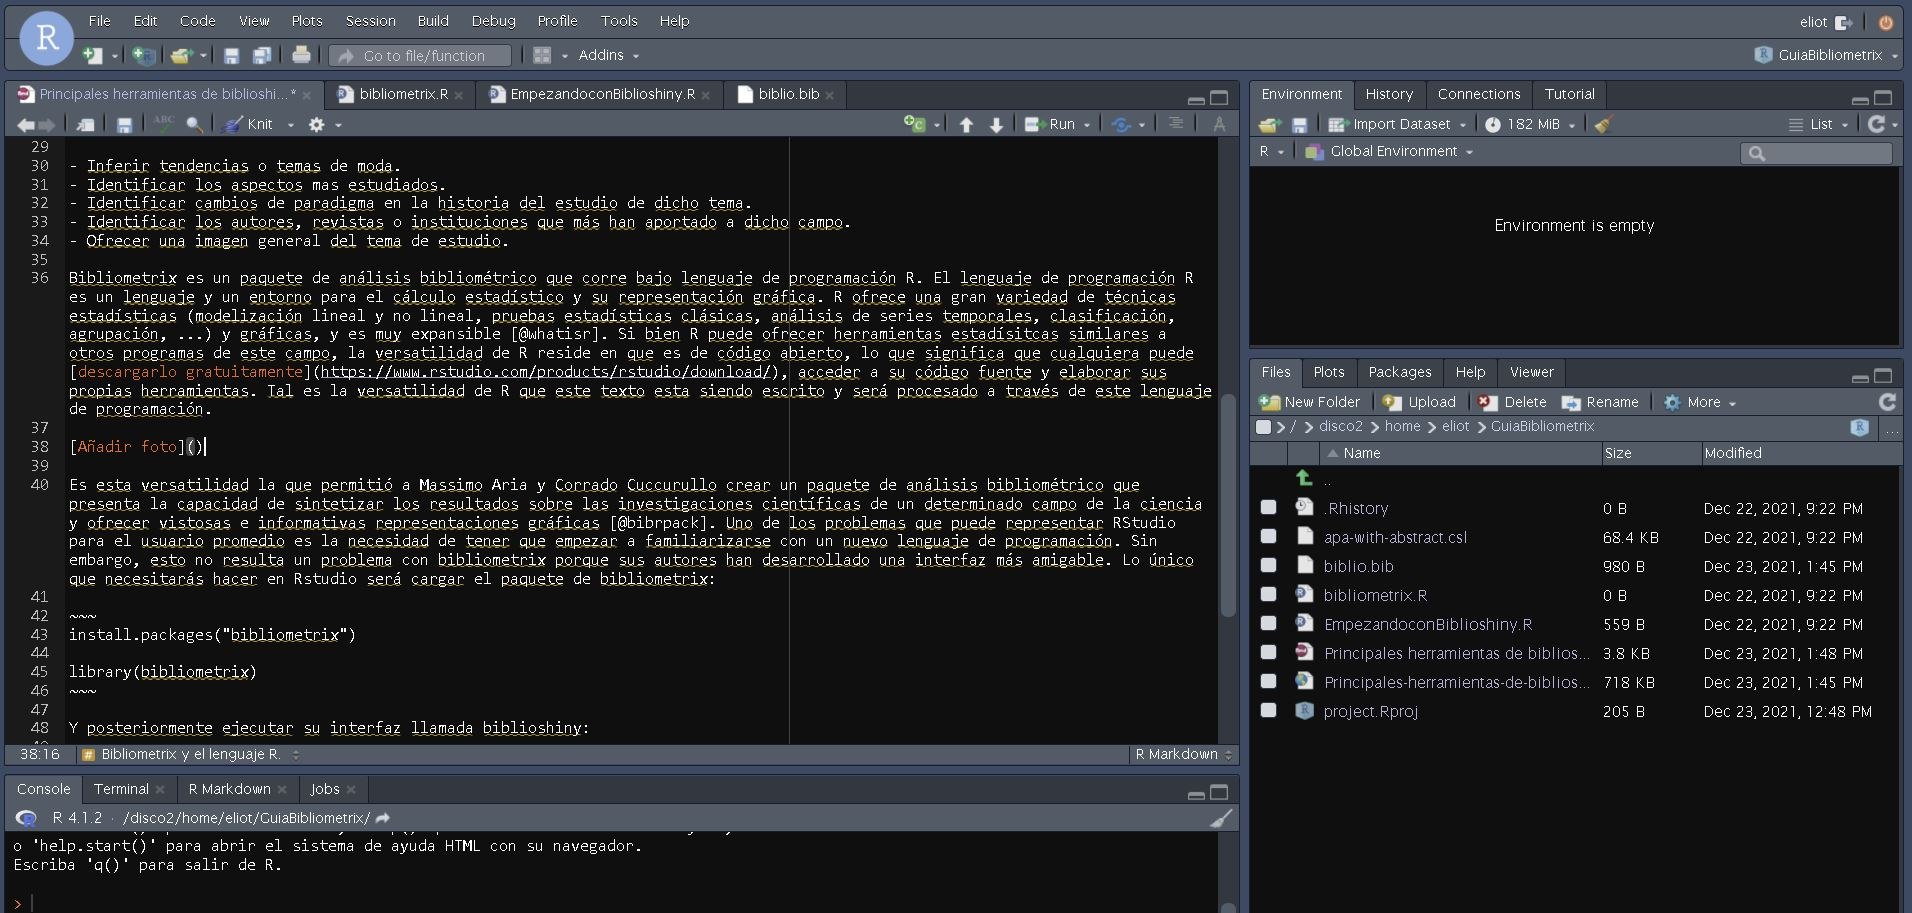
\includegraphics{rstudiointerfaz.JPG}
\caption{Interfaz de Rstudio}
\end{figure}

Es esta versatilidad la que permitió a Massimo Aria y Corrado Cuccurullo
crear un paquete de análisis bibliométrico que presenta la capacidad de
sintetizar los resultados sobre las investigaciones científicas de un
determinado campo de la ciencia y ofrecer vistosas e informativas
representaciones gráficas (\emph{Bibliometrix r Package}). Uno de los
problemas que puede representar RStudio para el usuario promedio es la
necesidad de tener que empezar a familiarizarse con un nuevo lenguaje de
programación. Sin embargo, esto no resulta un problema con bibliometrix
porque sus autores han desarrollado una interfaz más amigable. Lo único
que necesitarás hacer en Rstudio será cargar el paquete de bibliometrix
ejecutando los siguientes comandos en la consola:

\begin{verbatim}
install.packages("bibliometrix")

library(bibliometrix)
\end{verbatim}

Y posteriormente ejecutar su interfaz llamada biblioshiny:

\begin{verbatim}
biblioshiny()
\end{verbatim}

Cuando ejecutes este comando se te abrirá una pestaña de tu navegador
predeterminado con la siguiente interfaz:

\begin{figure}
\centering
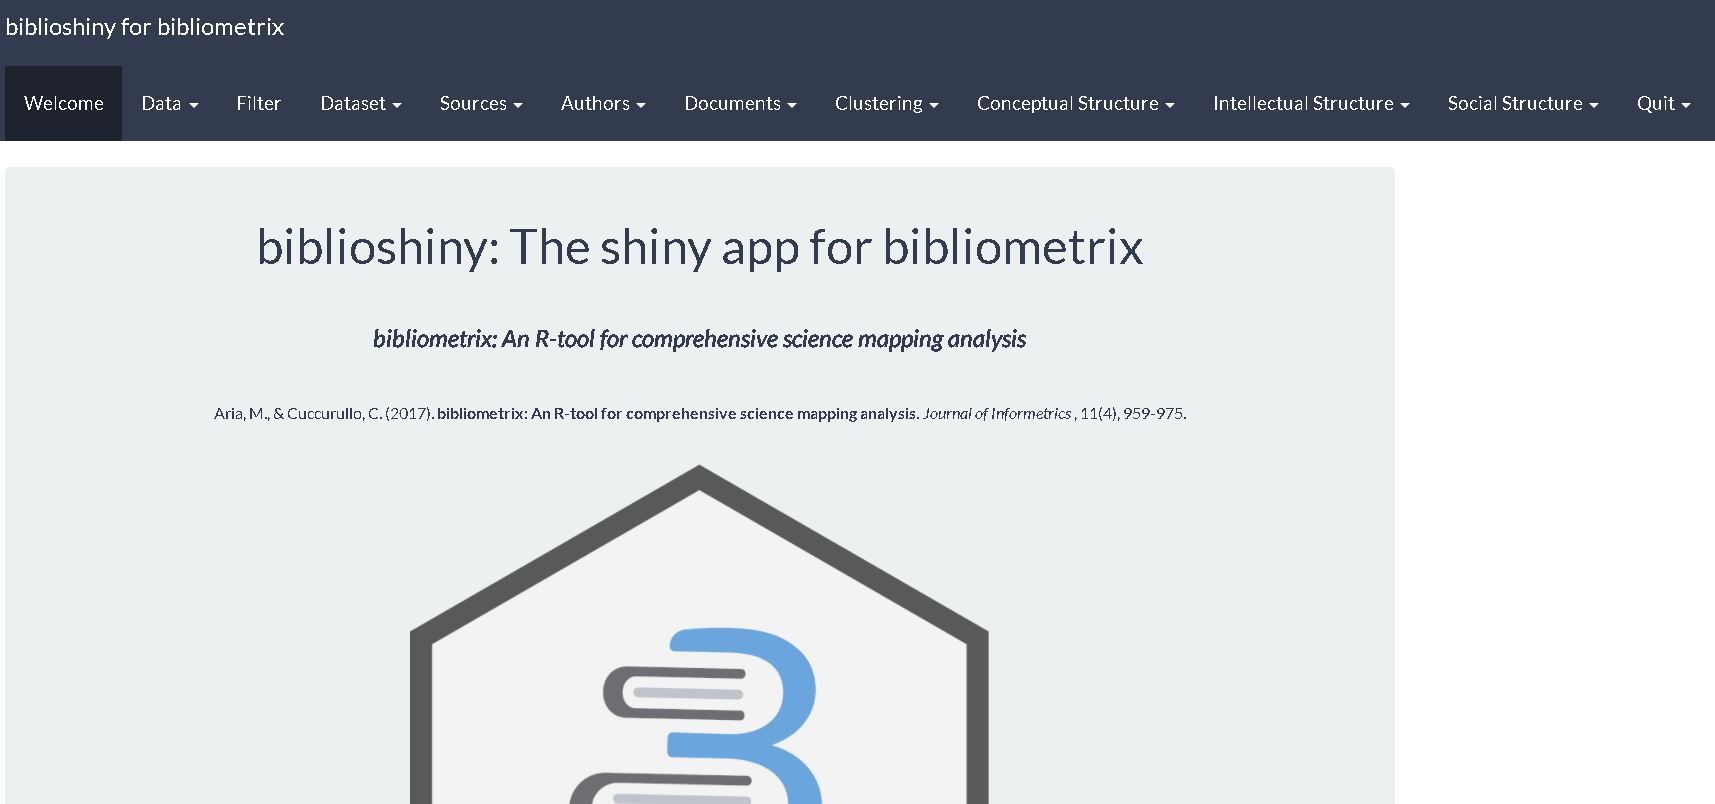
\includegraphics{biblioshinyinterfaz.JPG}
\caption{Interfaz de Biblioshiny}
\end{figure}

\hypertarget{bases-de-datos-y-como-cargarlos.}{%
\section{Bases de datos y como
cargarlos.}\label{bases-de-datos-y-como-cargarlos.}}

Utilizaremos para nuestra busqueda dos bases de datos: Scopus y Web of
Science (WOS). Scopus es más amigable con el usuario novato y da la
posibilidad de buscar tanto hacia adelante como hacia atrás a partir de
una cita concreta. Ambos buscadores almacenan información de artículos
de muy diversas disciplinas, lo que permite al investigador buscar
fácilmente fuera de su campo de estudio. WOS, por su parte, presenta una
mayor profunidad de cobertura, ya que la base de datos completa de WOS
se remonta a 1945 y la de Scopus a 1966. El uso de estas dos bases de
datos nos dará un volumen de información lo suficientemente completo
para nuestra investigación(Burnham, 2006).

A la hora de exportar los datos eligiremos el formato
\texttt{plaintext}(WOS) o \texttt{BibTeX}(Scopus), ya que son los que
menos problemas suele dar con bibliometrix. Aunque tenemos la
posibilidad de usar comandos para convertir nuestros datos a objetos que
puede manejar bibliometrix, partimos de la premisa de que queremos
trastocar con lenguaje de programación lo menos posible. Si quisieras
trastocar con distintos comandos para convertir formatos de las
distintas bases de datos puedes descargarte un manual
\href{https://www.bibliometrix.org/vignettes/Data-Importing-and-Converting.html}{aquí}.

\hypertarget{scopus.}{%
\subsection{Scopus.}\label{scopus.}}

Acudimos a \textbf{Scopus} y buscamos información sobre
\emph{Mutualistic Newtwork} en \textbf{Article Title, Absrtract and
Keywords}. El primer resultado nos arroja 406 resultados (TITLE-ABS-KEY
( ``mutualistic network'' )), pero realizaremos un filtrado a través del
apartado \textbf{Subject Area} de aquellas disciplinas que se salen de
nuestro campo de estudio, en nuestro caso queremos enfocarnos en el
estudio de los ecosistemas. Tras el filtrado, la busqueda avanzada queda
así:

TITLE-ABS-KEY ( ``mutualistic network'' ) AND ( EXCLUDE ( SUBJAREA ,
``MULT'' ) OR EXCLUDE ( SUBJAREA , ``PHYS'' ) OR EXCLUDE ( SUBJAREA ,
``IMMU'' ) OR EXCLUDE ( SUBJAREA , ``MATH'' ) OR EXCLUDE ( SUBJAREA ,
``COMP'' ) OR EXCLUDE ( SUBJAREA , ``ENGI'' ) OR EXCLUDE ( SUBJAREA ,
``NEUR'' ) OR EXCLUDE ( SUBJAREA , ``CHEM'' ) OR EXCLUDE ( SUBJAREA ,
``CENG'' ) OR EXCLUDE ( SUBJAREA , ``MATE'' ) OR EXCLUDE ( SUBJAREA ,
``MEDI'' ) OR EXCLUDE ( SUBJAREA , ``DECI'' ) OR EXCLUDE ( SUBJAREA ,
``PHAR'' ) OR EXCLUDE ( SUBJAREA , ``PSYC'' ) OR EXCLUDE ( SUBJAREA ,
``SOCI'' ) OR EXCLUDE ( SUBJAREA , ``ECON'' ) )\footnote{La búsqueda
  avanzada en Scopus implica el empleo de comandos de búsqueda basados
  en códigos, y está destinada a realizar búsquedas muy complejas, que
  exijan tal combinación de elementos, que las anteriores opciones de
  búsqueda no sean efectivas. Dado que Scopus no permite compartir
  busquedas a través de enlaces, comparto aquí el código de la busqueda
  avanzada. Con pegar este texto en la barra de busqueda deberías
  obtener los mismos resultados.}

Descargamos la bibliografía en formato \texttt{BibTeX} con toda la
información que nos permite Scopus (Citation information,
Bibliographical information, Abstract \& keywords, Funding details y
Other Information).

\hypertarget{web-of-science.}{%
\subsection{Web of Science.}\label{web-of-science.}}

Acudimos a \textbf{Web of Science} y buscamos información sobre
\href{https://www.webofscience.com/wos/alldb/summary/965e996b-ce32-4096-b23b-3d5fc1090cd3-1b146a07/relevance/1}{\emph{Mutualistic
Networks}} en \textbf{Topic}. Poseo cierto conocimiento previo sobre
este area, aportado gracias a artículos divulgativos que pueden
encontrarse facilmente. Esto me permite realizar un filtrado de los
resultados, ya que quiero enfocarme para mi TFG en el \emph{corpus}
teórico que ofrecen las redes mutualistas al estudio de los ecosistemas.
Para ello eliminé los resultados que parecen desviarse demasiado de este
tema, pero sin ser demasiado restrictivo, ya que el volumen de
resultados original (199) tampoco es demasiado grande y un filtrado
demasiado estricto podría dejarme con muy pocos datos para obtener
información relevante en el posterior análisis. Sin embargo, hay que
tener en cuenta que el filtrado de los datos inicial dependerá muchos de
los intereses y situación de cada investigador. La busqueda quedó
finalmente en
\href{https://www.webofscience.com/wos/alldb/summary/96d9e399-8558-49a7-bcc4-23b8a83d4a6e-1b14ad06/relevance/1}{160
resultados}.

\hypertarget{importar-datos-a-biblioshiny.}{%
\section{Importar datos a
biblioshiny.}\label{importar-datos-a-biblioshiny.}}

En la primera pestaña denominada \texttt{Data} podemos cargar los datos
a través de la opción \texttt{Import\ or\ Load\ Files}. La segunda
opción llamada \texttt{Gather\ Data\ using\ APIs} permite recopilar la
bibliografía directamente de las bases de datos correspondientes, pero
solo permite recoger datos de \textbf{Pubmed} y \textbf{Dimensions}, lo
que se sale de las bases de datos que queremos utilizar.

Para evitar tener que pasar por el uso de comandos de conversión en la
consola seleccionaremos en \textbf{Please, choose what to do} la opción
\texttt{Import\ raw\ files}, lo que significa que estamos importando
datos que descargamos directamente de la base de datos correspondiente,
sin realizar un proceso de conversión.

\textbf{ARREGLAR EL PROBLEMA DE IMPORTACION EN BIBLIOSHINY CON WOS}

\hypertarget{filtrar-datos-con-biblioshiny.}{%
\section{Filtrar datos con
Biblioshiny.}\label{filtrar-datos-con-biblioshiny.}}

Biblioshiny nos permite eliminar algunos datos de nuestra dependiendo de
nuestros intereses a través de la pestaña \texttt{Filter}. Entre las
opciones que nos ofrece nos permite filtrar por:

\begin{itemize}
\tightlist
\item
  Tipo de documento.
\item
  Año de publicación.
\item
  Total de citaciones.
\item
  Zonas de la ley de bradford.
\end{itemize}

En nuestro caso eliminaremos las fuentes de 2021 y 2022 ya que parecen
desvirtuar algunas gráficas y tendencias. Los últimos años de nuestra
muestra puede ser oportuno eliminarlos ya que son años susceptibles de
cambiar.

\hypertarget{principales-herramientas-de-biblioshiny.}{%
\section{Principales herramientas de
Biblioshiny.}\label{principales-herramientas-de-biblioshiny.}}

\hypertarget{informaciuxf3n-principal.}{%
\subsection{Información principal.}\label{informaciuxf3n-principal.}}

En \texttt{Dataset\textgreater{}Main\ Information} obtenemos información
cuantitativa sobre el set de artículos que hemos cargado a través de una
tabla.

\begin{longtable}[]{@{}ll@{}}
\toprule
biblioshiny for bibliometrix & \\
\midrule
\endhead
Description & Results \\
MAIN INFORMATION ABOUT DATA & \\
Timespan & 2002:2020 \\
Sources (Journals, Books, etc) & 84 \\
Documents & 242 \\
Average years from publication & 7.3 \\
Average citations per documents & 51.18 \\
Average citations per year per doc & 4.929 \\
References & 12555 \\
DOCUMENT TYPES & \\
article & 216 \\
book & 2 \\
book chapter & 8 \\
editorial & 1 \\
letter & 3 \\
note & 2 \\
review & 9 \\
short survey & 1 \\
DOCUMENT CONTENTS & \\
Keywords Plus (ID) & 881 \\
Author's Keywords (DE) & 720 \\
AUTHORS & \\
Authors & 690 \\
Author Appearances & 1010 \\
Authors of single-authored documents & 16 \\
Authors of multi-authored documents & 674 \\
AUTHORS COLLABORATION & \\
Single-authored documents & 20 \\
Documents per Author & 0.351 \\
Authors per Document & 2.85 \\
Co-Authors per Documents & 4.17 \\
Collaboration Index & 3.04 \\
\bottomrule
\end{longtable}

De esta tabla extraemos que tenemos un total de 242 documentos de los
años entre 2002 y 2020 y que son mayormente artículos científicos. Entre
los tipos de archivos minoritarios podemos destacar los capítulos de
libros y las revisiones, con 8 y 9 documentos respectivamente. La
mayoría de los autores se encuentran en documentos con múltiples autores
y muchos de ellos presente coautoría, con 4.17 coautores por documento.

\hypertarget{producciuxf3n-cientuxedfica-anual.}{%
\subsection{Producción científica
anual.}\label{producciuxf3n-cientuxedfica-anual.}}

En \texttt{Data\textgreater{}Annual\ Scientific\ Production} nos muestra
una gráfica que enfrenta número de artículos por año. Esta gráfica es
muy ilustrativa del desarrollo en popularidad del tema de estudio.

\begin{figure}
\centering
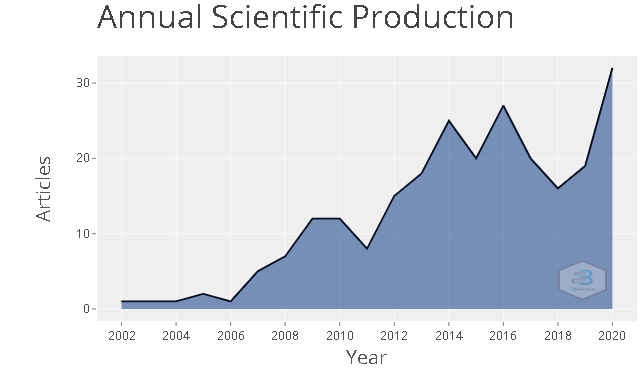
\includegraphics{AnnualScientificProduction.png}
\caption{Diagrama de la producción científica anual}
\end{figure}

El diagrama nos permite observar que el tema de estudio presenta unos
años iniciales de producción científica modesta, con uno o dos artículos
por año entre 2002 y 2006. Posteriormente se produce la explosión, con
picos productivos en 2009, 2014, 2016 y 2020, con 12, 25, 27 y 32
documentos respectivamente. Por lo tanto, es probable que en esos años
previos encontremos algún o algunos artículos muy citados que resultaran
ser la semilla de todo un campo de estudio. Al examinar estos años
encontramos dos artículos muy citados:

\begin{itemize}
\tightlist
\item
  Invariant properties in coevolutionary networks of plant--animal
  links. Jordano, Bascompte y Olessen. 2003. Con 546 citas.
\item
  Geographic patterns in plant--pollinator mutualistic networks. Olessen
  y Jordano. 2002. Con 395 citas. Un buen punto de partida para nuestra
  lectura podrían ser estos dos artículos.
\end{itemize}

A la izquierda nos encontramos un ratio de crecimiento anual del 21.23\%
que es calculado utilizando la fórmula para el Compound annual growth
rate (CAGR) utilizado mayormente en economía.

\hypertarget{media-de-citaciones-al-auxf1o.}{%
\subsection{Media de citaciones al
año.}\label{media-de-citaciones-al-auxf1o.}}

En la pestaña
\texttt{Dataset\textgreater{}Average\ Citations\ per\ Year} encontramos
un diagrama con el número de citaciones promedio que recibió nuestras
citaciones promedio cada año. En nuestros datos podemos observar que
existen picos de citaciones en los primeros años de las publicaciones,
lo que nos indica que existen artículos muy influyentes en dichos años.

\begin{figure}
\centering
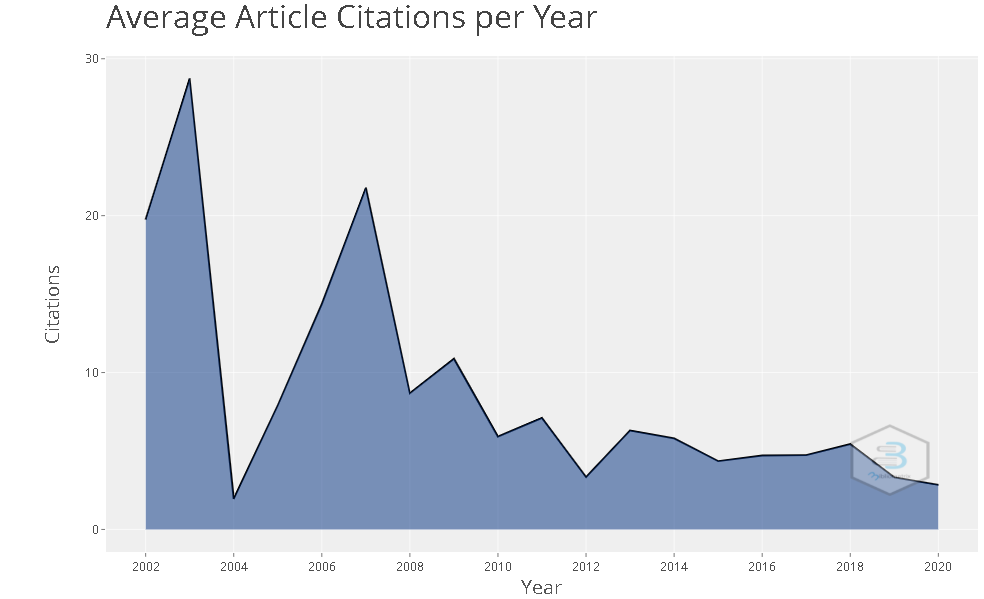
\includegraphics{AverageCitationsPerYear.png}
\caption{Diagrama del promedio de citaciones al año}
\end{figure}

\hypertarget{diagrama-de-tres-campos.}{%
\subsection{Diagrama de tres campos.}\label{diagrama-de-tres-campos.}}

En la pestaña \texttt{Dataset\textgreater{}Three-Fields\ Plot}
encontramos el diagrama de tres campos, una representación grafíca que
permite mostrar en tres columnas separadas algunos de los campos
asociados a cualquier documento (autores, palabras clave, titulos,
fuentes etc.) e interconectarlos en función de si presentan una relación
visible en nuestra muestra bibliográfica. Por ejemplo, un autor puede
ser conectados con los artículos que cita, con las palabras clave que
utiliza o con las fuentes en las que aparece. El menú desplegable de la
izquierda nos permite elegir los elementos que ponemos en cada campo, lo
que se presta a realizar múltiples combinaciones para observar las
distintas redes. Propongo como ejemplo la representación de
\texttt{References} en la izquierda, \texttt{Authors} en el centro y
\texttt{Keywords\ Plus} en la derecha. Recomiendo reducir el número de
unidades por campo a 10, para reducir la cantidad de datos representados
y que resulte menos confuso.

\begin{figure}
\centering
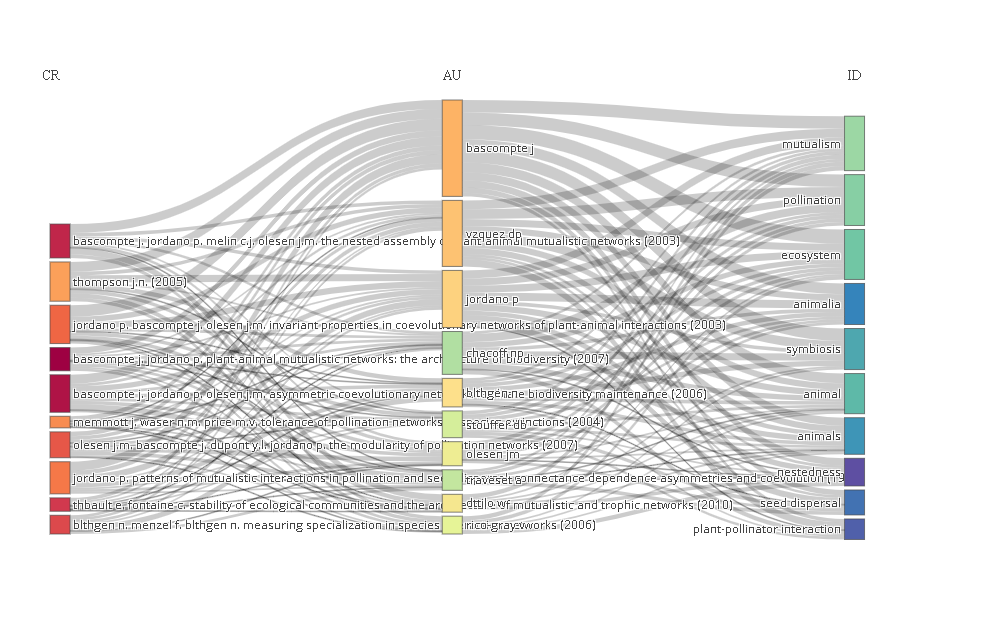
\includegraphics{ThreeFieldsPlot.png}
\caption{Diagrama de tres campos representando a la izquierda las
referencias, en el centro los autores y a la derecha palabras clave
plus}
\end{figure}

Esta representación nos permite observar de un vistazo cuales son las
referencias mas citadas, con qué autores conecta y qué palabras clave
tiene relacion. Los puntos débiles de esta combinación es que la
longitud de los títulos de las referncias solapan con con el campo
central, lo que resulta confuso. Recomiendo interactuar con el diagrama
colocando el ratón sobre las distintas unidades representadas, ya que
con esta acción se acentúan las interacciones de dichos elementos y
permite sacar mejores conclsuiones.

\hypertarget{fuentes.}{%
\subsection{Fuentes.}\label{fuentes.}}

Una fuente es una revista, libro, capítulo de libro, conferencia o
cualquiera que sea el origen de dicha información. El análisis de las
fuentes puede ser interesante para observar cuales son las que más
impacto tienen en nuestro campo de estudio y puede guiar busquedas
futuras. Identificar cuales son las fuentes más relevantes puede hacerse
siguiendo múltiples estrategias, biblioshiny nos ofrece 5 herramientas
distintas para medir distintas características de lo que se puede
considerar una fuente importante.

\hypertarget{fuentes-muxe1s-relevantes.}{%
\subsubsection{Fuentes más
relevantes.}\label{fuentes-muxe1s-relevantes.}}

En la pestaña \texttt{Sources\textgreater{}Most\ relevant\ Sources} nos
muestra la cantidad de documentos que presentan las fuentes de nuestra
muesta bibliográfica.

\begin{figure}
\centering
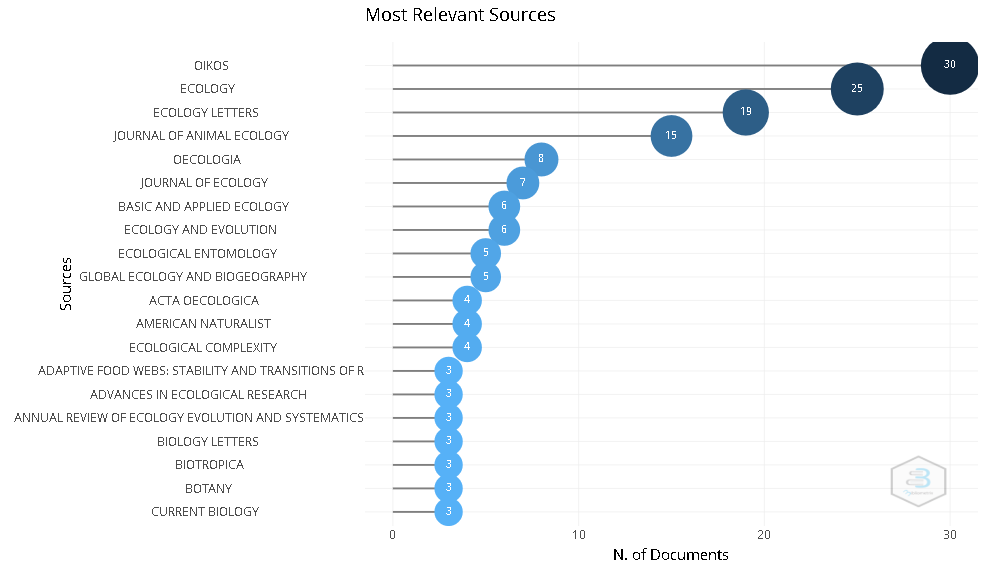
\includegraphics{MostRelevantSources.png}
\caption{Diagrama del número de documentos de cada una de las fuentes}
\end{figure}

Tomando como criterio de importancia el número de documentos, las
revistas OIKOS, ECOLOGY, ECOLOGY LETTERS y JOURNAL OF ANIMAL ECOLOGY son
las fuentes con mas relevancia.

\hypertarget{fuentes-localmente-muxe1s-citadas.}{%
\subsubsection{Fuentes localmente más
citadas.}\label{fuentes-localmente-muxe1s-citadas.}}

En la pestaña \texttt{Sources\textgreater{}Most\ Local\ Cited\ Sources}
nos muestra un diagrama con las fuentes localmente más citadas. Las
fuentes localmente más citadas son aquellas que aparecen en la
bibliografía de los documentos de nuestra muestra bibliográfica.

\begin{figure}
\centering
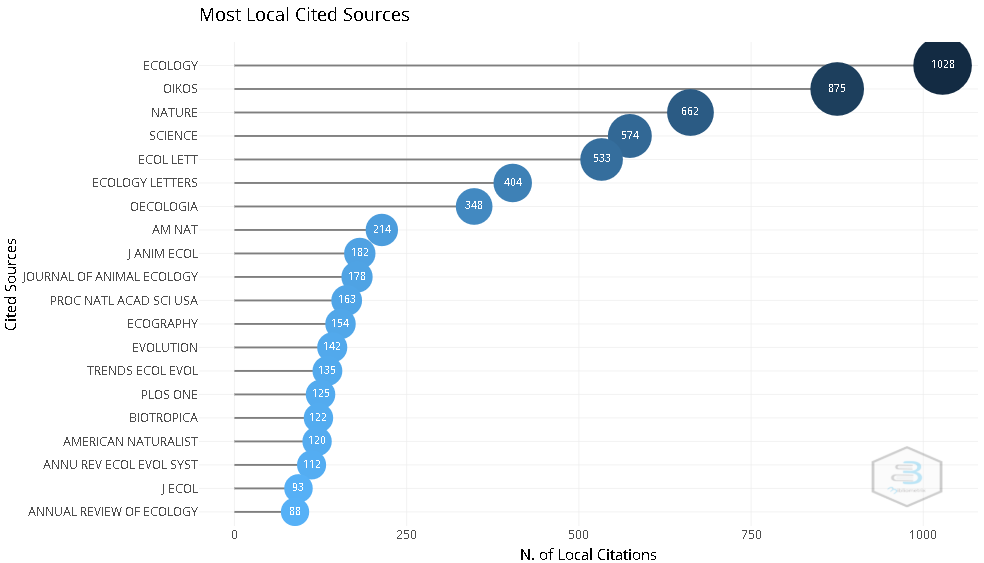
\includegraphics{MostLocalCitedSources.png}
\caption{Diagrama de las fuentes localmente mas citadas}
\end{figure}

En el aspecto de las citas ECOLOGY gana a OIKOS y se introducen revistas
que no aparecían antes en el análisis como NATURE o SCIENCE. Esto puede
deberse a que son revistas científicas de alto impacto a lo largo de
muchos campos de estudio distintos, por lo que los autores las conocen,
leen sus artículos regularmente y las acaban citando en sus trabajos,
pero dado que apenas poseen artículos relacionados con nuestro tema es
posible que no debamos tenerlas en cuenta.

\hypertarget{ley-de-bradford.}{%
\subsubsection{Ley de bradford.}\label{ley-de-bradford.}}

Podemos realizar un cálculo de las resvistas que forman parte del
``núcleo'' a través de la ley de bradford, que se encuentra en
\texttt{Sources\textgreater{}Bradford´s\ law}.

En biblishiny puedes aplicar la ley de bradford en la pestaña
\texttt{Sources\textgreater{}Bradford\textquotesingle{}s\ Law}.

\begin{figure}
\centering
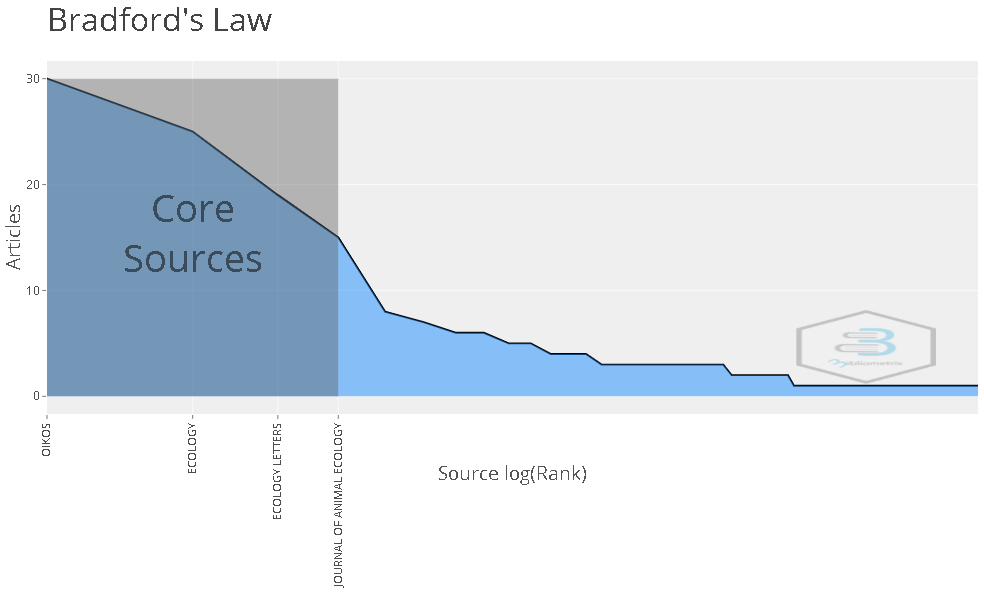
\includegraphics{BradfordsLaw.png}
\caption{Diagrama de la Ley de Bradford}
\end{figure}

La pestaña \texttt{plot} nos ofrece una tabla con la misma información
representada en el diagrama. Podemos observar como la cantidad de
fuentes en las zonas 2 y 3 es considerablemente mayor que las de la zona
1, lo que valida las conclusiones de Bradford. La siguiente tabla
muestra las fuentes que se encuentran en la zona 1, y por lo tanto a las
que deberemos prestar mas atención:

\begin{longtable}[]{@{}lllll@{}}
\toprule
& & & & \\
\midrule
\endhead
SO & Rank & Freq & cumFreq & Zone \\
OIKOS & 1 & 32 & 32 & Zone 1 \\
ECOLOGY & 2 & 27 & 59 & Zone 1 \\
ECOLOGY LETTERS & 3 & 22 & 81 & Zone 1 \\
JOURNAL OF ANIMAL ECOLOGY & 4 & 17 & 98 & Zone 1 \\
\bottomrule
\end{longtable}

\hypertarget{impacto-de-las-fuentes.}{%
\subsubsection{Impacto de las fuentes.}\label{impacto-de-las-fuentes.}}

Biblioshiny nos permite medir el impacto de las fuentes a través de 4
parámetros:

\begin{itemize}
\tightlist
\item
  Índice \(h\)
\item
  Índice \(g\)
\item
  Índice \(m\)
\item
  Total de citas
\end{itemize}

Podemos aplicar el cálculo de estos cuatro parámetros mediante el menú
desplegable ´Impact measure´. Si elegimos el índice \(h\) nos aparece un
diagrama con 20 revistas, pero debido a que a partir de la décimo
segunda nos aparecen un total de 10 revistas con índice \(h\) de 3,
reducimos el total de revistas que aparecen a 12 para sobrecargar menos
con información redundante.

\begin{figure}
\centering
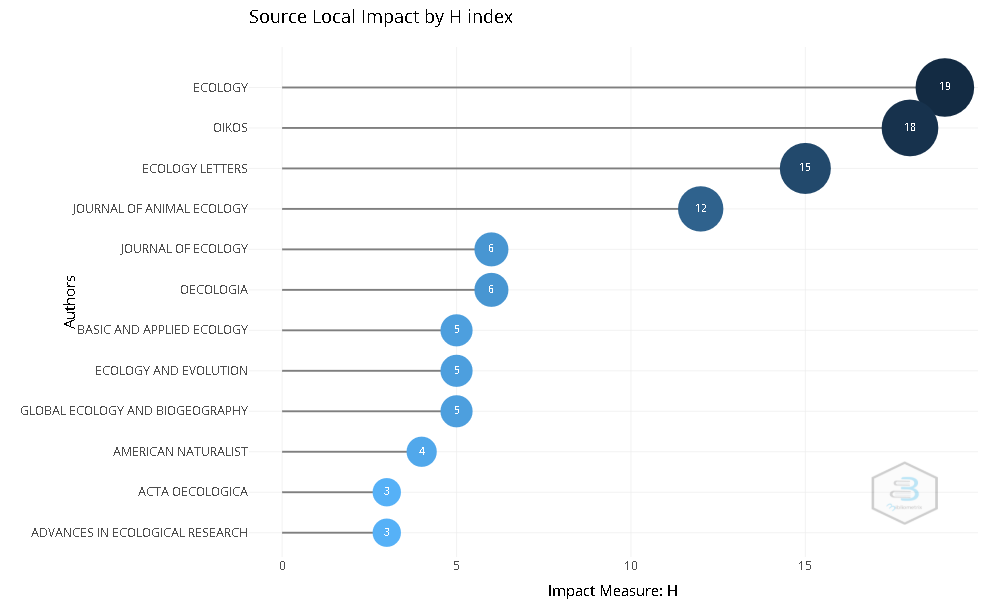
\includegraphics{SourceImpactByHIndex.png}
\caption{Diagrama índice \(h\) de revistas}
\end{figure}

El índice \(h\) de las fuentes, así como la ley de bradford, nos vuelve
a indicar que las fuentes a las que debemos prestar mas antención son
ECOLOGY, OIKOS, ECOLOGY LETTERS y JOURNAL OF ANIMAL ECOLOGY. La ley de
bradford nos informaba de que estas revistas son las que forman parte
del núcleo de la investigación, mientras que el índice \(h\) nos informa
de que, además, son las que tienen más impacto.

Si elegimos \texttt{G-Index}, obtendremos un diagrama similar al
obtenido cuando medíamos el índice \(h\) pero para el índice \(g\).

\begin{figure}
\centering
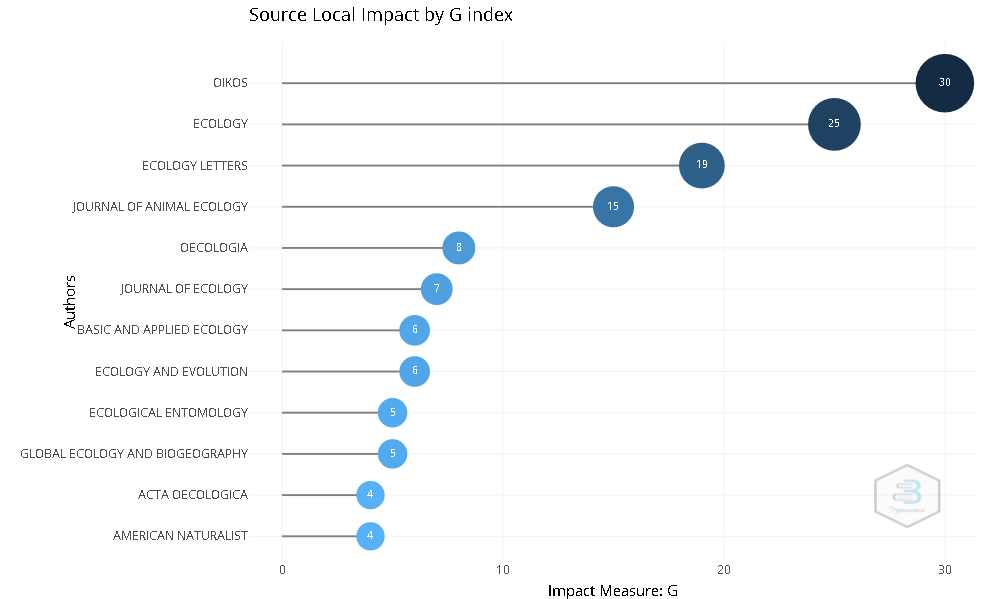
\includegraphics{SourceImpactByGIndex.png}
\caption{Diagrama índice \(g\) de revistas}
\end{figure}

Podemos observar que ahora las dos revistas más citadas aparecen más
separadas entre sí, mientras que las menos citadas no han cambiado
mucho. Hemos ganado precisión para discernir entre las revistas más
citadas, mientras que con el índice \(h\) ECOLOGY tiene más impacto que
OIKOS sin mucha diferencia, con el índice \(g\) observamos que OIKOS
tiene más impacto con bastante más diferencia. Probablemente, OIKOS
tiene algunos artículos muy citados que hacen que gane la carrera en el
índice \(g\).

Si elegimos \texttt{M-Index}, obtebdremos ahora el diagrama para el
índice \(m\) de impacto. Existe una fuente con un nombre muy largo que
nos comprime el diagrama hacia la derecha, como este es el último
reducimos el númeoro de fuentes representadas a 11 para obtener un
diagrama más apaisado.

\begin{figure}
\centering
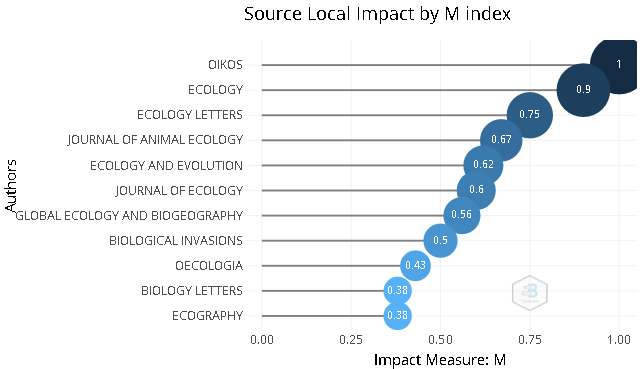
\includegraphics{SocurceImpactByMIndex.png}
\caption{Diagrama índice \(m\) de revistas}
\end{figure}

El diagrama sobre el índice \(m\) no nos da información relevante sobre
las fuentes más importantes, ya que su posición en los puestos altos de
la lista no cambia. Sin embargo, si observamos que las revistas
secundarias de menos impacto si sufren cambios significativos en su
posición en la lista. De todas formas, debido a que estas revistas
secundarias no serán de nuestro interés en nuestra investigación, no
tendremos en cuenta estos leves cambios.

\begin{longtable}[]{@{}lllllll@{}}
\toprule
biblioshiny for bibliometrix & & & & & & \\
\midrule
\endhead
Element & h\_index & g\_index & m\_index & TC & NP & PY\_start \\
ECOLOGY & 19 & 25 & 0.904761904761905 & 2014 & 25 & 2002 \\
OIKOS & 18 & 30 & 1 & 1116 & 30 & 2005 \\
ECOLOGY LETTERS & 15 & 19 & 0.75 & 2101 & 19 & 2003 \\
JOURNAL OF ANIMAL ECOLOGY & 12 & 15 & 0.666666666666667 & 1395 & 15 &
2005 \\
JOURNAL OF ECOLOGY & 6 & 7 & 0.6 & 155 & 7 & 2013 \\
OECOLOGIA & 6 & 8 & 0.428571428571429 & 138 & 8 & 2009 \\
BASIC AND APPLIED ECOLOGY & 5 & 6 & 0.3125 & 171 & 6 & 2007 \\
ECOLOGY AND EVOLUTION & 5 & 6 & 0.625 & 83 & 6 & 2015 \\
GLOBAL ECOLOGY AND BIOGEOGRAPHY & 5 & 5 & 0.555555555555556 & 208 & 5 &
2014 \\
AMERICAN NATURALIST & 4 & 4 & 0.266666666666667 & 170 & 4 & 2008 \\
ACTA OECOLOGICA & 3 & 4 & 0.25 & 34 & 4 & 2011 \\
ADVANCES IN ECOLOGICAL RESEARCH & 3 & 3 & 0.230769230769231 & 141 & 3 &
2010 \\
\bottomrule
\end{longtable}

Resumidamente podemos decir que las cuatro revistas mas importantes de
nuestra muestra son ECOLOGY, OIKOS, ECOLOGY LETTERS Y JOURNAL OF ANIMAL
ECOLOGY. El índice \(g\) nos ha dado información interesante sobre
OIKOS, ya que probablemente presente un artículo muy citado que nos sea
útil en nuestra investigación. El índice \(m\) no nos ha dado
información relevante sobre las revistas mas importantes.

\hypertarget{dinuxe1mica-de-las-fuentes.}{%
\subsubsection{Dinámica de las
fuentes.}\label{dinuxe1mica-de-las-fuentes.}}

En la pestaña \texttt{Sources\textgreater{}Source\ Dynamics} encontramos
un diagrama que nos muestra la dinámica de las fuentes a partir de la
representación acumulada o por año de la cantidad de artículos. En el
menú desplegable \texttt{Ocurrences} podemos alternar entre las dos
representaciones.

\begin{figure}
\centering
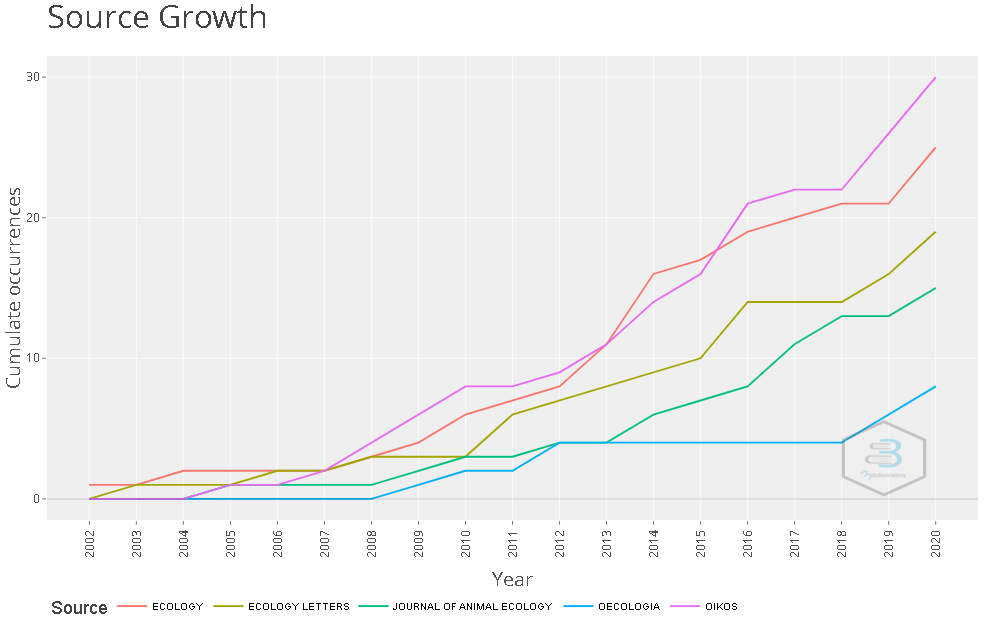
\includegraphics{SourceGorwth.png}
\caption{Diagrama del crecimiento acumulado en número de artículos de
las fuentes}
\end{figure}

Las cuatro revistas más importantes siguen siendo las ya mencionadas.
OIKOS y ECOLOGY presentan un largo historial de interés sobre este tema
desde los años 2007 y 2008, donde parecen encontrarse a la carrera por
quien posee mas artículos. Actualmente lleva la delantera OIKOS con 30
artículos y le sigue ECOLOGY con 25.

\hypertarget{autores.}{%
\subsection{Autores.}\label{autores.}}

La búsqueda de los autores más relevantes puede seguirse bajo varios
criterios que observaremos a continuación. Conocer a los autores más
importantes de una disciplina es uno de los aspcetos más importantes a
la hora de conocer un determinado campo de estudio.

\hypertarget{autores-muxe1s-relevantes.}{%
\subsubsection{Autores más
relevantes.}\label{autores-muxe1s-relevantes.}}

En la pestaña \texttt{Authors\textgreater{}Most\ Relevant\ Authors}
podemos realizar 3 análisis distintos relacionados con la relevancia de
los autores. Estos análisis se pueden alternar a partir del menú
deplegable de la izquierda \texttt{Frequency\ measure}, donde podemos
elegir entre representar número de documentos, porcentaje del total de
documentos o frecuencia fraccionalizada.

\begin{figure}
\centering
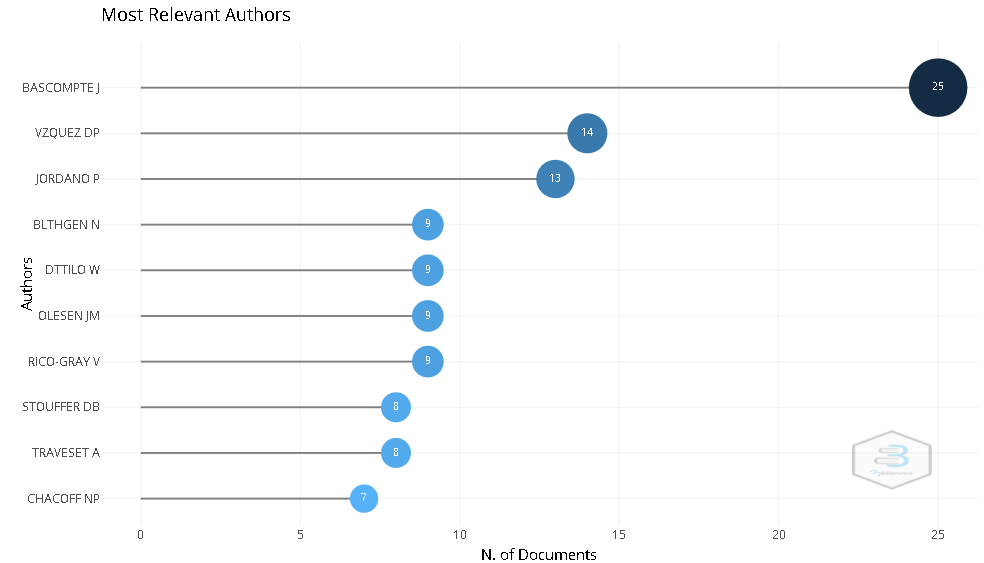
\includegraphics{MostRelevantAuthorsND.png}
\caption{Diagrama de los autores mas relevantes por número de
documentos}
\end{figure}

Bascompte, Vazquez y Jordano son los autores más productivos, por lo que
puede ser interesante prestarles atención. Con la frecuencia
fraccionalizada estos autores principales no cambian su posición, por lo
que podemos decir que además de presentar muchos artículos, estos
presentan pocos coautores, de lo que se puede deducir que probablemente
realizaron una alta contribución a sus respectivos trabajos.

\hypertarget{autores-localmente-muxe1s-citados.}{%
\subsubsection{Autores localmente más
citados.}\label{autores-localmente-muxe1s-citados.}}

En la pestaña
\texttt{Authors\textgreater{}Most\ Local\ Cited\ Documents} encontramos
cuales son los autores más citados dentro de nuestra muestra
bibliográfica.

\begin{figure}
\centering
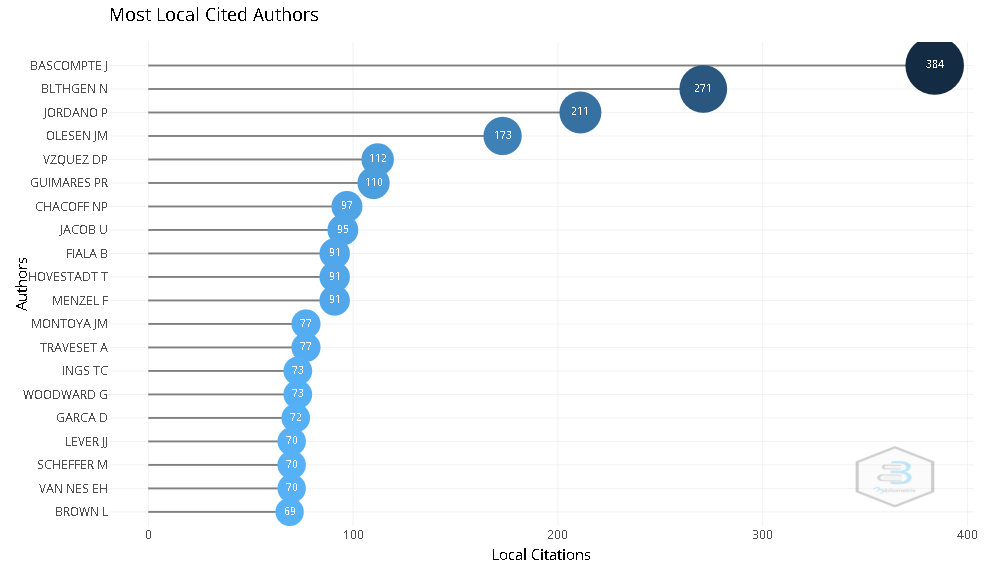
\includegraphics{MostLocalCitedAuthors.png}
\caption{Diagrama de los autores localmente más citados}
\end{figure}

Cuando observamos los autores localmente más citados, dos autores entran
a la palestra: Blthgen y Olessen. Puede ser que, aunque estos autores no
tienen tanta repercusión cuando contamos las citas simples, si tienen
repercusión dentro de nuestra muestra y sería interesante investigar su
trayectoria.

\hypertarget{producciuxf3n-de-los-autores-a-lo-largo-del-tiempo.}{%
\subsubsection{Producción de los autores a lo largo del
tiempo.}\label{producciuxf3n-de-los-autores-a-lo-largo-del-tiempo.}}

En la pestaña
\texttt{Authors\textgreater{}Author\textquotesingle{}s\ Production\ over\ Time}
se representan los 20 autores más antiguos. Cada una de las líneas
representa el recorrido de los autores y las burbujas representan su
producción científica. La posición de las burbujas indican el año en que
se produjeron los artículos, el tamaño representa la cantidad de
artículos producidos ese año y la intensidad del color la cantidad de
citas recibidas.

\begin{figure}
\centering
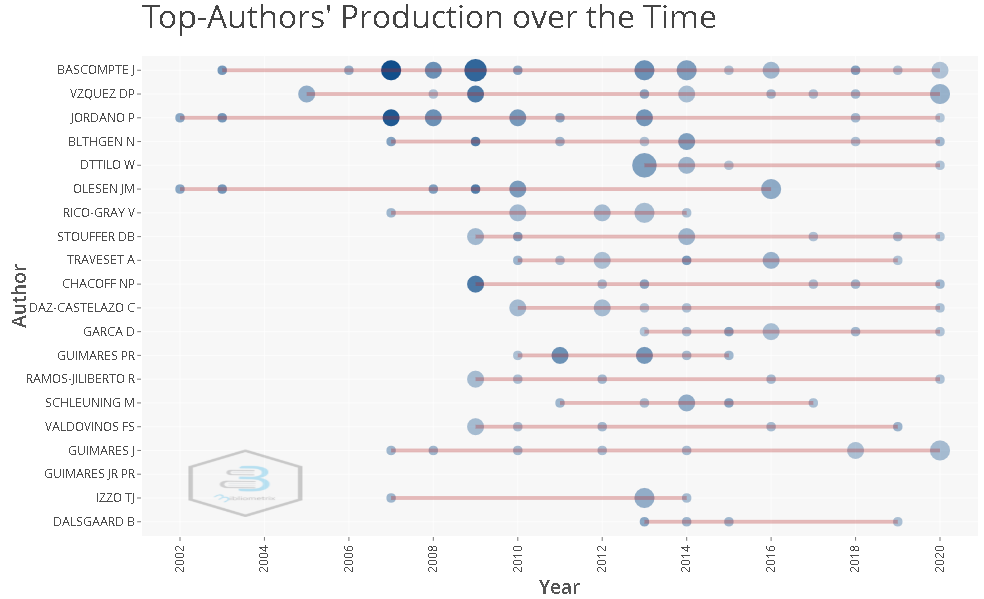
\includegraphics{TopAuthorsProductionOverTime.png}
\caption{Diagrama de la producción científica a lo largo del tiempo}
\end{figure}

En este diagrama es interesante enfocarse en cuales son las burbujas más
grandes y con el azul más intenso. Los autores que hasta ahora eran más
importantes según otros análisis repiten en este diagrama siendo los mas
productivos. Sin embargo, es curioso observar que otro autor al que no
habíamos tenido en cuenta, a saber Chacoff, presenta un artículo muy
citado en 2009 y el resto de su trayectoría es menos productiva. Para
observar cuales son los autores más producitvos conviene observar la
tabla de la pestaña \texttt{Table-Top\ Authors\ Production\ Per\ Year} y
ordenar a los autores de mayor a menor citas por año.

\begin{longtable}[]{@{}lllll@{}}
\toprule
biblioshiny for bibliometrix & & & & \\
\midrule
\endhead
Author & year & freq & TC & TCpY \\
BASCOMPTE J & 2007 & 3 & 1144 & 71.500 \\
JORDANO P & 2007 & 2 & 1044 & 65.250 \\
BASCOMPTE J & 2009 & 4 & 805 & 57.500 \\
CHACOFF NP & 2009 & 2 & 634 & 45.286 \\
VZQUEZ DP & 2009 & 2 & 634 & 45.286 \\
BLTHGEN N & 2009 & 1 & 596 & 42.571 \\
OLESEN JM & 2009 & 1 & 596 & 42.571 \\
BASCOMPTE J & 2008 & 2 & 481 & 32.067 \\
JORDANO P & 2008 & 2 & 481 & 32.067 \\
BASCOMPTE J & 2013 & 3 & 315 & 31.500 \\
\bottomrule
\end{longtable}

\hypertarget{ley-de-lotkas.}{%
\subsubsection{Ley de lotka´s.}\label{ley-de-lotkas.}}

En la pestaña
\texttt{Authors\textgreater{}Lotka\textquotesingle{}s\ Law} podemos
medir la productividad de los autores de nuestra muestra y observar si
nuestro modelo se ajusta a Ley de Lotka.

\begin{figure}
\centering
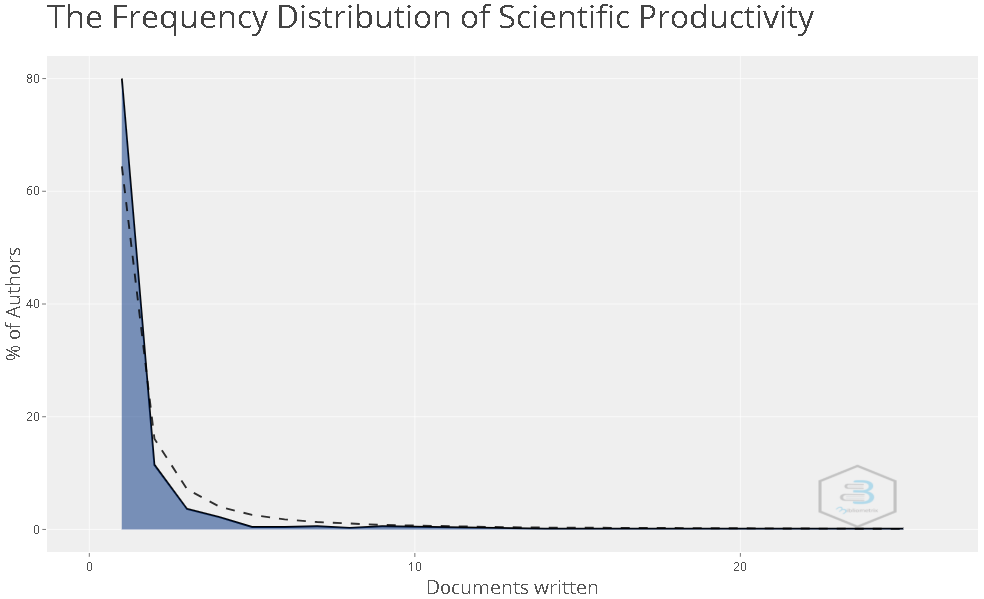
\includegraphics{LotkasLaw.png}
\caption{Diagrama de la ley de Lotka}
\end{figure}

La línea oscura es la ley de Lotka según nuestros datos y la linea
punteada es la distribución teórica. El 80\% de los autores han
publicado solo un artículo sobre el tema, la función se extiende hacia
la derecha, donde encontraríamos a los autores mas productivos que son
una minoría, en este caso al menos 5 documentos.

\begin{longtable}[]{@{}lll@{}}
\toprule
biblioshiny for bibliometrix & & \\
\midrule
\endhead
Documents written & N. of Authors & Proportion of Authors \\
1 & 552 & 0.800 \\
2 & 79 & 0.114 \\
3 & 25 & 0.036 \\
4 & 15 & 0.022 \\
5 & 3 & 0.004 \\
6 & 3 & 0.004 \\
7 & 4 & 0.006 \\
8 & 2 & 0.003 \\
9 & 4 & 0.006 \\
13 & 1 & 0.001 \\
14 & 1 & 0.001 \\
25 & 1 & 0.001 \\
\bottomrule
\end{longtable}

\hypertarget{impacto-de-los-autores.}{%
\subsubsection{Impacto de los autores.}\label{impacto-de-los-autores.}}

Biblioshiny nos permite medir el impacto de los autores con la pestaña
\texttt{Authors\textgreater{}Author\ Local\ Impact} y podemos medir 4
parámetros:

\begin{itemize}
\tightlist
\item
  Índice \(h\)
\item
  Índice \(g\)
\item
  Índice \(m\)
\item
  Total de citas
\end{itemize}

\begin{figure}
\centering
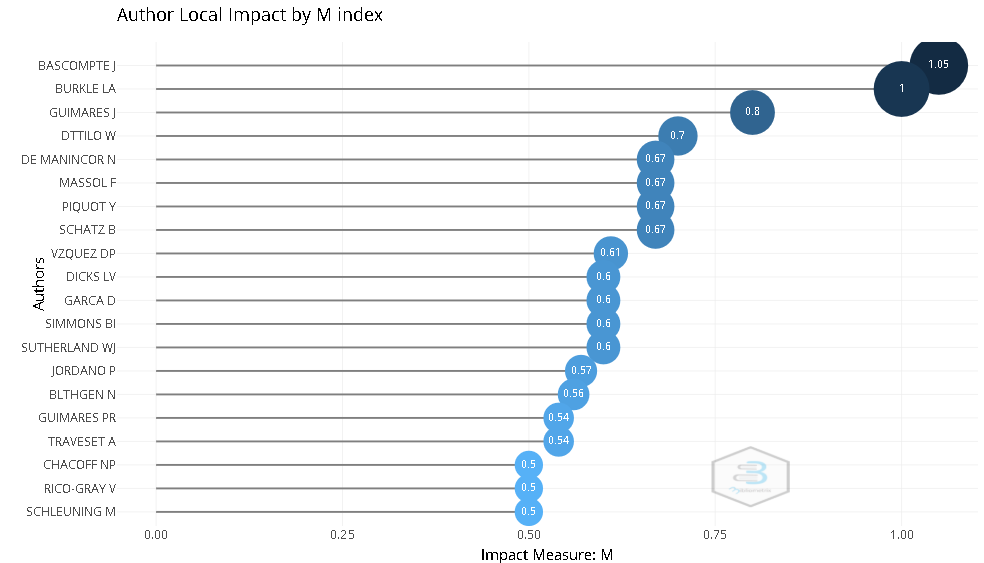
\includegraphics{AuthorsLocalImpactByMIndex.png}
\caption{Diagrama del índice \(m\) de los autores}
\end{figure}

Podemos aplicar el cálculo de estos cuatro parámetros mediante el menú
desplegable \texttt{Impact\ measure}. El índice \(h\) y \(g\) nos da
información sobre lo que ya sabíamos, es decir, que Bascompte, Vazque y
Jordano son los autores más relevantes. Sin embargo, hay que tener en
cuenta que el índice \(m\) propone a otros autores por delante, como
Burkle o Guimares, lo que puede ser una señal de que algunos de los
autores mas importantes según los indices \(h\) y \(g\) se encuentren
sobrerrepresentados por presentar una trayectoría más larga.

\hypertarget{pauxedses-de-los-correspondientes-autores.}{%
\subsubsection{Países de los correspondientes
autores.}\label{pauxedses-de-los-correspondientes-autores.}}

En la pestaña
\texttt{Authros\textgreater{}Corresponding\ Author´s\ country} podemos
generar un diagrama donde se representan los paises mas productivos en
función del número de documentos. En naranja aparecen la cantidad de
documentos donde al menos uno de sus coautores es de un país diferente
(MCP, \emph{Multiple Countries Publication}) y en azul la cantidad de
documentos cuyos coautores son todos del mismo país (SCP, \emph{Single
Country Publication}).

\begin{figure}
\centering
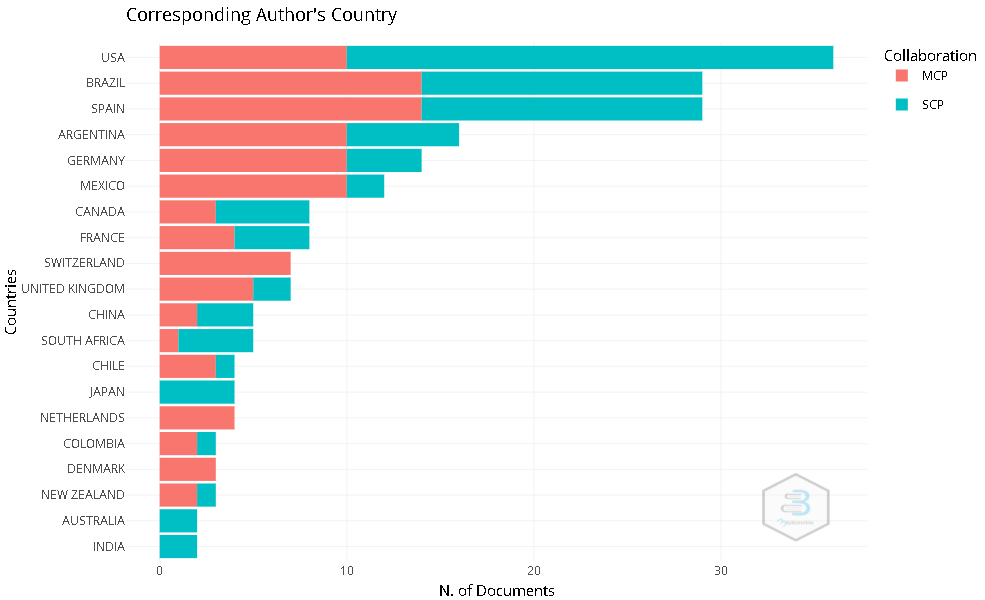
\includegraphics{CorrespondingAuthorsCountry.png}
\caption{Diagrama de la producción científica por paises}
\end{figure}

Podemos observar que Estados Unidos, Brasil y España son los paises más
productivos, seguidos de Argentina, Alemania y México. 3 de los paises
más productivos son hispanohablantes, lo cuál es a destacar. Todos los
paises presentan niveles de contribución con otros paises bastante
altos, destacando Argentina, Alemania y México.

\hypertarget{producciuxf3n-cientuxedfica-de-los-pauxedses.}{%
\subsubsection{Producción científica de los
países.}\label{producciuxf3n-cientuxedfica-de-los-pauxedses.}}

Otra manera de observar la producción científica por países es
observarla representada en un Mapa Mundi. Para ello podemos acudir a la
pestaña \texttt{Authors\textgreater{}Country\ Scientific\ Production}
donde te ofrece un Mapa Mundi donde los países mas productivos aparecen
coloreados en tonos de azul más intenso.

\begin{figure}
\centering
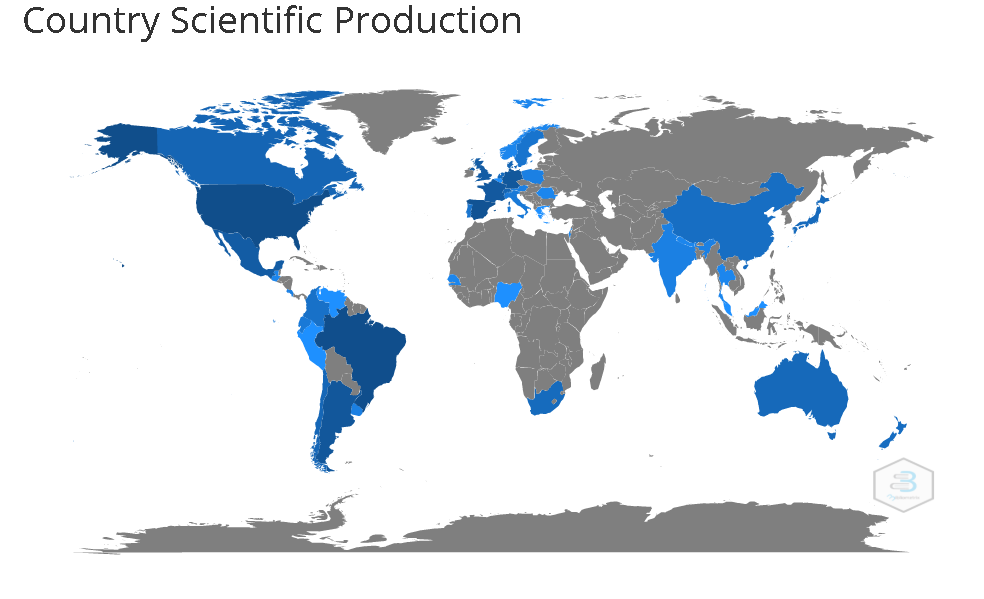
\includegraphics{CountryScientificProduction.png}
\caption{Mapamundi de la producción científica por paises.}
\end{figure}

\hypertarget{pauxedses-muxe1s-citados.}{%
\subsubsection{Países más citados.}\label{pauxedses-muxe1s-citados.}}

En la pestaña \texttt{Authors\textgreater{}Most\ Cited\ Countries} nos
muestra un diagrama con los países mas citados.

\begin{figure}
\centering
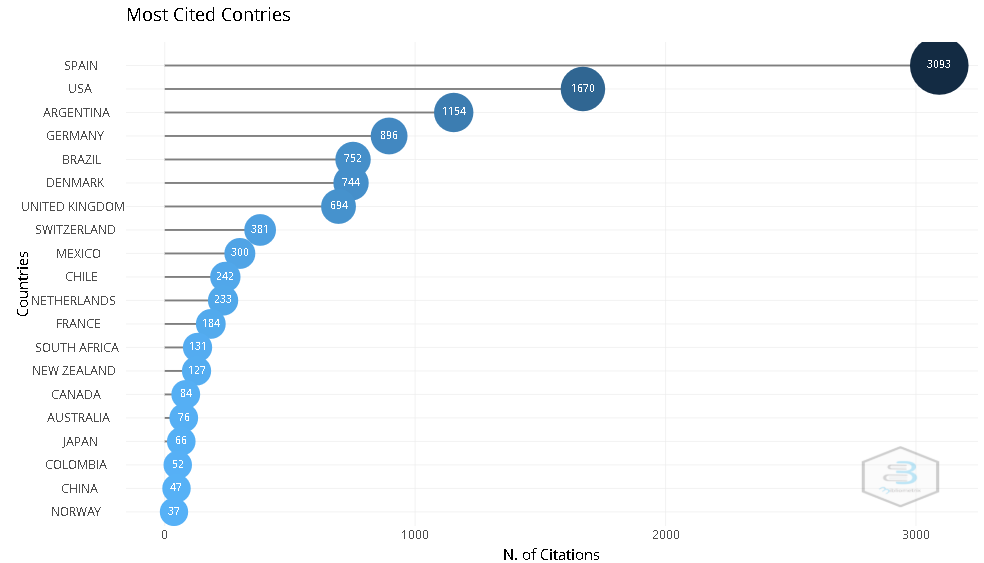
\includegraphics{MostCitedSources.png}
\caption{Diagrama de los paises mas citados}
\end{figure}

Estados Unidos y Brasil son paises más productivos, pero España resulta
ser la más citada, probablemente resultado de que los autores mas
citados provienen de este país.

\hypertarget{documentos.}{%
\subsection{Documentos.}\label{documentos.}}

\hypertarget{documentos-globalmente-muxe1s-citados.}{%
\subsubsection{Documentos globalmente más
citados.}\label{documentos-globalmente-muxe1s-citados.}}

Una primera aproximación a averiguar cuales son los artículos más
relevantes puede ser observar cuales son los artículos más citados. En
\texttt{Documents\textgreater{}Most\ Global\ Cited\ Documents}
encontrarás un diagrama de barras con los artículos más citados.

\begin{figure}
\centering
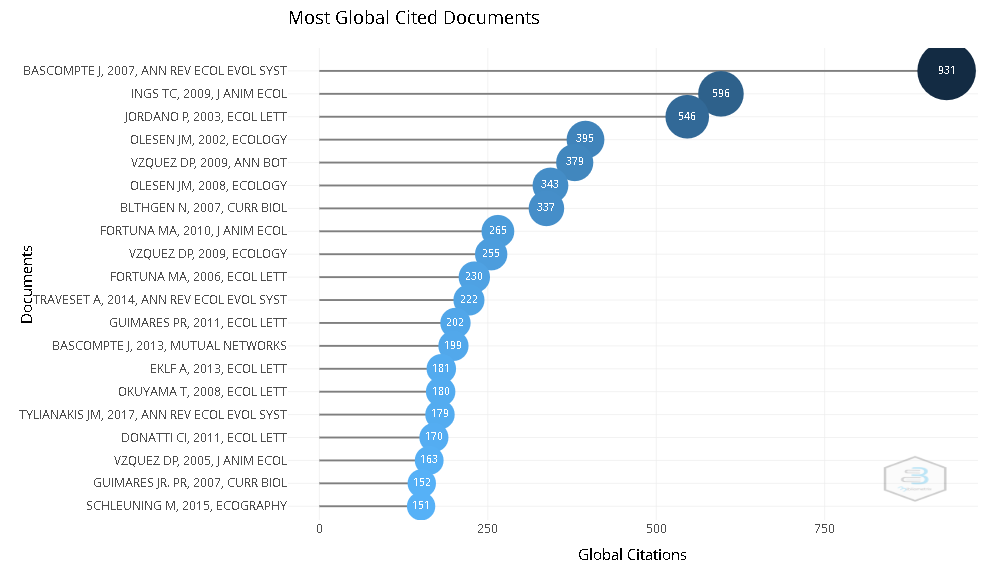
\includegraphics{MostGlobalCitedDocuments.png}
\caption{Diagrama de barras de los artículos mas citados.}
\end{figure}

Los artículos globalmente mas citados son Bascompte 2007 como el mas
citado de sobra con 931 citas. Le sigue Ings TC 2009 y Jordano 2003 con
596 y 546 citas respectivamente.

\begin{longtable}[]{@{}
  >{\raggedright\arraybackslash}p{(\columnwidth - 8\tabcolsep) * \real{0.32}}
  >{\raggedright\arraybackslash}p{(\columnwidth - 8\tabcolsep) * \real{0.35}}
  >{\raggedright\arraybackslash}p{(\columnwidth - 8\tabcolsep) * \real{0.12}}
  >{\raggedright\arraybackslash}p{(\columnwidth - 8\tabcolsep) * \real{0.09}}
  >{\raggedright\arraybackslash}p{(\columnwidth - 8\tabcolsep) * \real{0.11}}@{}}
\toprule
biblioshiny for bibliometrix & & & & \\
\midrule
\endhead
Paper & DOI & Total Citations & TC per Year & Normalized TC \\
BASCOMPTE J, 2007, ANN REV ECOL EVOL SYST &
10.1146/annurev.ecolsys.38.091206.095818 & 931 & 58.1875 & 2.85058 \\
INGS TC, 2009, J ANIM ECOL & 10.1111/j.1365-2656.2008.01460.x & 596 &
42.5714 & 4.21450 \\
JORDANO P, 2003, ECOL LETT & 10.1046/j.1461-0248.2003.00403.x & 546 &
27.3000 & 1.00000 \\
OLESEN JM, 2002, ECOLOGY &
10.1890/0012-9658(2002)083{[}2416:GPIPPM{]}2.0.CO;2 & 395 & 18.8095 &
1.00000 \\
VZQUEZ DP, 2009, ANN BOT & 10.1093/aob/mcp057 & 379 & 27.0714 &
2.68002 \\
OLESEN JM, 2008, ECOLOGY & 10.1890/07-0451.1 & 343 & 22.8667 &
2.82139 \\
BLTHGEN N, 2007, CURR BIOL & 10.1016/j.cub.2006.12.039 & 337 & 21.0625 &
1.03184 \\
FORTUNA MA, 2010, J ANIM ECOL & 10.1111/j.1365-2656.2010.01688.x & 265 &
20.3846 & 3.72802 \\
VZQUEZ DP, 2009, ECOLOGY & 10.1890/08-1837.1 & 255 & 18.2143 &
1.80318 \\
FORTUNA MA, 2006, ECOL LETT & 10.1111/j.1461-0248.2005.00868.x & 230 &
13.5294 & 1.00000 \\
TRAVESET A, 2014, ANN REV ECOL EVOL SYST &
10.1146/annurev-ecolsys-120213-091857 & 222 & 24.6667 & 4.77625 \\
GUIMARES PR, 2011, ECOL LETT & 10.1111/j.1461-0248.2011.01649.x & 202 &
16.8333 & 2.58147 \\
BASCOMPTE J, 2013, MUTUAL NETWORKS & NA & 199 & 19.9000 & 3.50489 \\
EKLF A, 2013, ECOL LETT & 10.1111/ele.12081 & 181 & 18.1000 & 3.18787 \\
OKUYAMA T, 2008, ECOL LETT & 10.1111/j.1461-0248.2007.01137.x & 180 &
12.0000 & 1.48061 \\
TYLIANAKIS JM, 2017, ANN REV ECOL EVOL SYST &
10.1146/annurev-ecolsys-110316-022821 & 179 & 29.8333 & 7.55274 \\
DONATTI CI, 2011, ECOL LETT & 10.1111/j.1461-0248.2011.01639.x & 170 &
14.1667 & 2.17252 \\
VZQUEZ DP, 2005, J ANIM ECOL & 10.1111/j.1365-2656.2005.00992.x & 163 &
9.0556 & 1.21190 \\
GUIMARES JR. PR, 2007, CURR BIOL & 10.1016/j.cub.2007.09.059 & 152 &
9.5000 & 0.46540 \\
SCHLEUNING M, 2015, ECOGRAPHY & 10.1111/ecog.00983 & 151 & 18.8750 &
4.95082 \\
\bottomrule
\end{longtable}

\hypertarget{documentos-localmente-muxe1s-citados.}{%
\subsubsection{Documentos localmente más
citados.}\label{documentos-localmente-muxe1s-citados.}}

En la pestaña
\texttt{Documents\textgreater{}Most\ Local\ Cited\ Documents}
encontramos el diagrama de los documentos localmente más citados.

\begin{figure}
\centering
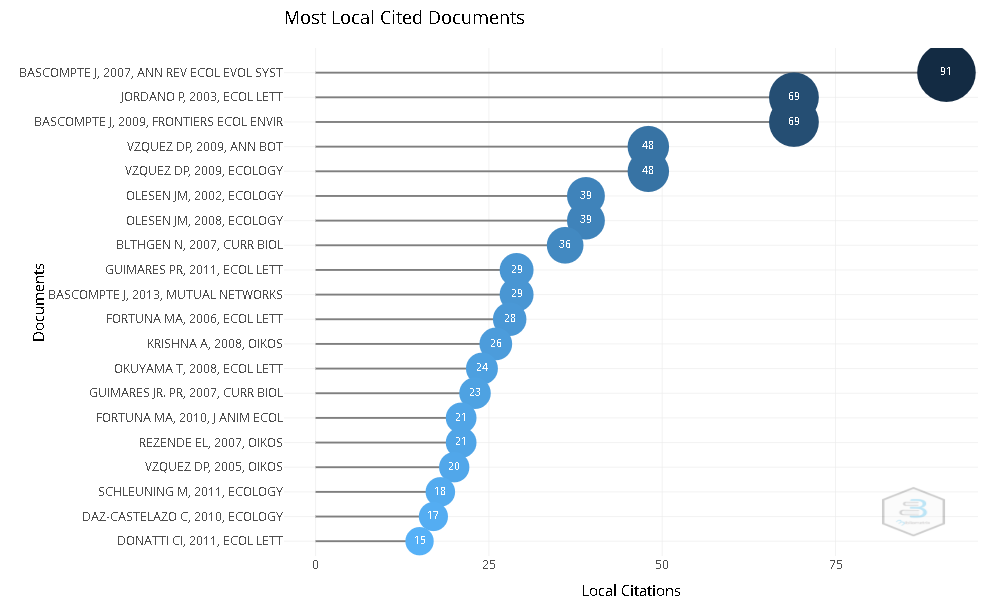
\includegraphics{MostLocalCitedDocuments.png}
\caption{Diagrama de los documentos localmente mas citados}
\end{figure}

Bascompte 2007 sigue siendo de los documentos más citados, lo que nos
indica que es un documento importante, muy citado tanto por documentos
externos a nuestra colección como por documentos de nuestra colección.
Ingst 2009 desaparece de los documentos localmente mas citados y es
sustituido por documentos de otros autores. Jordano 2003 aparece entre
los documentos mas citados ahora en segundo puesto, lo que nos indica
que tambien es un documento importante. Otros artículos como Vazquez
2009 y Olessen 2002 repiten también entre los documentos más citados.

\begin{longtable}[]{@{}
  >{\raggedright\arraybackslash}p{(\columnwidth - 14\tabcolsep) * \real{0.21}}
  >{\raggedright\arraybackslash}p{(\columnwidth - 14\tabcolsep) * \real{0.24}}
  >{\raggedright\arraybackslash}p{(\columnwidth - 14\tabcolsep) * \real{0.03}}
  >{\raggedright\arraybackslash}p{(\columnwidth - 14\tabcolsep) * \real{0.08}}
  >{\raggedright\arraybackslash}p{(\columnwidth - 14\tabcolsep) * \real{0.09}}
  >{\raggedright\arraybackslash}p{(\columnwidth - 14\tabcolsep) * \real{0.08}}
  >{\raggedright\arraybackslash}p{(\columnwidth - 14\tabcolsep) * \real{0.14}}
  >{\raggedright\arraybackslash}p{(\columnwidth - 14\tabcolsep) * \real{0.14}}@{}}
\toprule
biblioshiny for bibliometrix & & & & & & & \\
\midrule
\endhead
Document & DOI & Year & Local Citations & Global Citations & LC/GC Ratio
(\%) & Normalized Local Citations & Normalized Global Citations \\
BASCOMPTE J, 2007, ANN REV ECOL EVOL SYST &
10.1146/annurev.ecolsys.38.091206.095818 & 2007 & 91 & 931 & 9.77 & 2.61
& 2.85 \\
JORDANO P, 2003, ECOL LETT & 10.1046/j.1461-0248.2003.00403.x & 2003 &
69 & 546 & 12.64 & 1.00 & 1.00 \\
BASCOMPTE J, 2009, FRONTIERS ECOL ENVIR & 10.1890/080026 & 2009 & 69 &
96 & 71.88 & 4.02 & 0.68 \\
VZQUEZ DP, 2009, ANN BOT & 10.1093/aob/mcp057 & 2009 & 48 & 379 & 12.66
& 2.80 & 2.68 \\
VZQUEZ DP, 2009, ECOLOGY & 10.1890/08-1837.1 & 2009 & 48 & 255 & 18.82 &
2.80 & 1.80 \\
OLESEN JM, 2002, ECOLOGY &
10.1890/0012-9658(2002)083{[}2416:GPIPPM{]}2.0.CO;2 & 2002 & 39 & 395 &
9.87 & 1.00 & 1.00 \\
OLESEN JM, 2008, ECOLOGY & 10.1890/07-0451.1 & 2008 & 39 & 343 & 11.37 &
2.60 & 2.82 \\
BLTHGEN N, 2007, CURR BIOL & 10.1016/j.cub.2006.12.039 & 2007 & 36 & 337
& 10.68 & 1.03 & 1.03 \\
GUIMARES PR, 2011, ECOL LETT & 10.1111/j.1461-0248.2011.01649.x & 2011 &
29 & 202 & 14.36 & 3.01 & 2.58 \\
BASCOMPTE J, 2013, MUTUAL NETWORKS & 2013 & 29 & 199 & 14.57 & 5.17 &
3.50 & \\
FORTUNA MA, 2006, ECOL LETT & 10.1111/j.1461-0248.2005.00868.x & 2006 &
28 & 230 & 12.17 & 1.00 & 1.00 \\
KRISHNA A, 2008, OIKOS & 10.1111/j.1600-0706.2008.16540.x & 2008 & 26 &
138 & 18.84 & 1.73 & 1.14 \\
OKUYAMA T, 2008, ECOL LETT & 10.1111/j.1461-0248.2007.01137.x & 2008 &
24 & 180 & 13.33 & 1.60 & 1.48 \\
GUIMARES JR. PR, 2007, CURR BIOL & 10.1016/j.cub.2007.09.059 & 2007 & 23
& 152 & 15.13 & 0.66 & 0.47 \\
FORTUNA MA, 2010, J ANIM ECOL & 10.1111/j.1365-2656.2010.01688.x & 2010
& 21 & 265 & 7.92 & 3.27 & 3.73 \\
REZENDE EL, 2007, OIKOS & 10.1111/j.0030-1299.2007.16029.x & 2007 & 21 &
113 & 18.58 & 0.60 & 0.35 \\
VZQUEZ DP, 2005, OIKOS & 10.1111/j.0030-1299.2005.13619.x & 2005 & 20 &
106 & 18.87 & 1.21 & 0.79 \\
SCHLEUNING M, 2011, ECOLOGY & 10.1890/09-1842.1 & 2011 & 18 & 111 &
16.22 & 1.87 & 1.42 \\
DAZ-CASTELAZO C, 2010, ECOLOGY & 10.1890/08-1883.1 & 2010 & 17 & 86 &
19.77 & 2.65 & 1.21 \\
DONATTI CI, 2011, ECOL LETT & 10.1111/j.1461-0248.2011.01639.x & 2011 &
15 & 170 & 8.82 & 1.56 & 2.17 \\
\bottomrule
\end{longtable}

\hypertarget{espectroscopuxeda-de-las-referencias.}{%
\subsubsection{Espectroscopía de las
referencias.}\label{espectroscopuxeda-de-las-referencias.}}

En la pestaña \texttt{Documentos\textgreater{}Reference\ Spectroscopy}
podemos realizar una espectroscopía de los años de publicación de las
referencias citadas. Existe una referencia citada de 1713 que desvirtúa
el gráfico. Para conseguir que el gráfico esté menos comprimido hacia la
izuquierda localizamos el siguiente año más citado y hacemos el análisis
a partir de él. En nuestro caso elegimos 1859, que tiene un total de 5
referencias citadas, y lo especificamos en el menú de la izquierda en
\texttt{TimeSlice\textgreater{}Starting\ Year}.

\begin{figure}
\centering
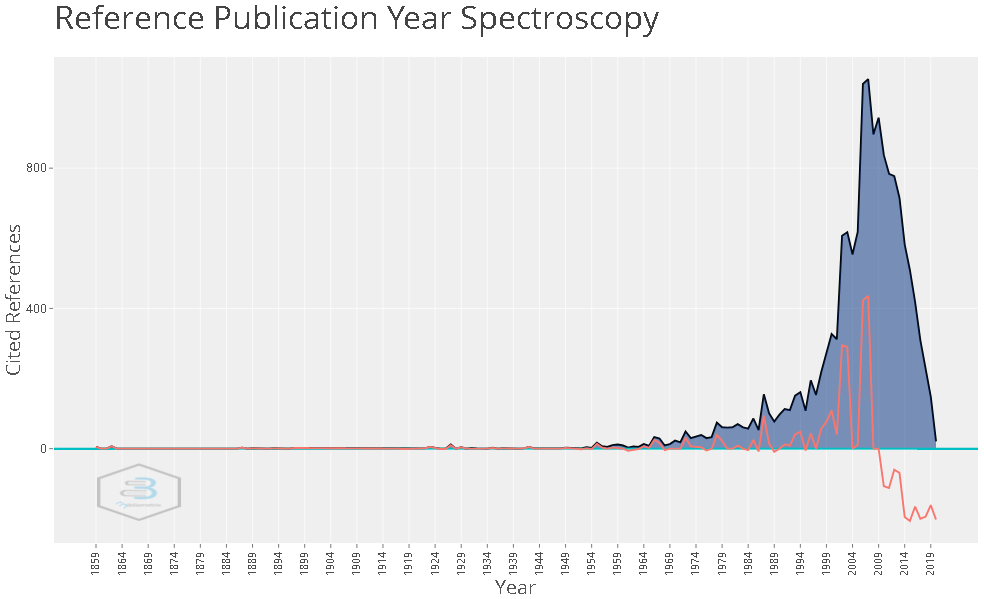
\includegraphics{ReferencePublicationYearSpectroscopy.png}
\caption{Espectroscopía de las referncias}
\end{figure}

A través de esta espectroscopía es interesante observar los picos, ya
que representan años donde se publicaron referencias que fueron muy
citadas. Nuestro conjunto de artículos proviene de los años 2002:2020,
por lo que para localizar las racies de un tema puede ser interesante
observar los artículos mas citados de los años anteriores a 2002, porque
serán las influencias de nuestro campo de estudio. Entre 1955:2000
podemos localizar 11 picos cuyas referencias sería interesante revisar
para localizar las fuentes de nuestro tema.

\begin{longtable}[]{@{}lll@{}}
\toprule
biblioshiny for bibliometrix & & \\
\midrule
\endhead
Year & Citations & diffMedian5 \\
2000 & 327 & 109 \\
1995 & 108 & -5 \\
1994 & 161 & 48 \\
1993 & 151 & 41 \\
1987 & 155 & 94 \\
1985 & 86 & 25 \\
1978 & 74 & 39 \\
1972 & 49 & 31 \\
1966 & 33 & 25 \\
1955 & 17 & 14 \\
\bottomrule
\end{longtable}

\hypertarget{palabras-mas-frecuentes.}{%
\subsubsection{Palabras mas
frecuentes.}\label{palabras-mas-frecuentes.}}

En la pestaña \texttt{Documents\textgreater{}Most\ Frequent\ Words}
aparecen las palabras que más aparecen en nuestros documentos. Entre los
parámetros que pueden modificarse en el menu de la izquierda tenemos:

\begin{itemize}
\item
  El campo: Las palabras mas frecuentes pueden aparecer en distintos
  campos de un artículo como las Keywords Plus, las Keywords del autor,
  el título o el resumen. En el título y el resumen puede elegirse si se
  quieren grupos de una, dos o tres palabras (N-Grams).
\item
  La cantidad de palabras que aparecen en el diagrama.
\end{itemize}

\begin{figure}
\centering
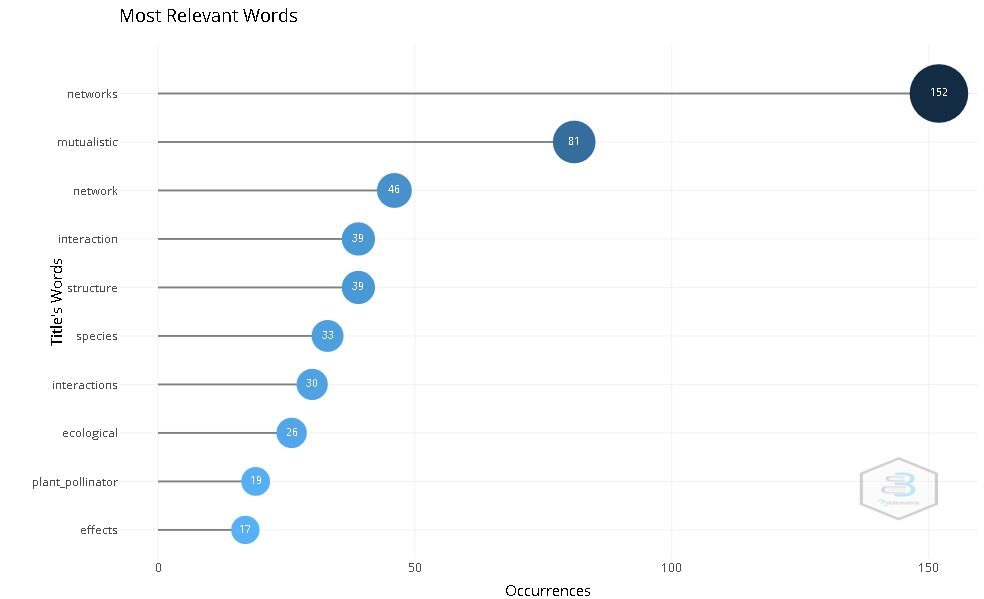
\includegraphics{MostFrequentWords.png}
\caption{Diagrama de palabras más frecuentes}
\end{figure}

Por ejemplo, entre las palabras más frecuentes de los títulos
encontramos \emph{networks}, \emph{mutualism} e \emph{interaction}.
Puede llamarnos la atención que aparezca la palabra
\emph{plant-polinator}, lo que puede darnos una pista de uno de los
tipos de interacciones ecológicas que toman protagonismo dentro del
campo de las redes mutualistas.

\hypertarget{nube-de-palabras.}{%
\subsubsection{Nube de palabras.}\label{nube-de-palabras.}}

Biblioshiny nos ofrece una herramienta para dar cuenta de las palabras
mas utilizadas de una manera más vistosa, estas son las nubes de
palabras. Podemos acceder a nubes de palabras mediante la pestaña
\texttt{Documents\textgreater{}WordCloud}. Entre las opciones que
podemos configurar está:

\begin{itemize}
\item
  El campo: Las palabras mas frecuentes pueden aparecer en distintos
  campos de un artículo como las Keywords Plus, las Keywords del autor,
  el título o el resumen. En el título y el resumen puede elegirse si se
  quieren grupos de una, dos o tres palabras (N-Grams).
\item
  Número de palabras que aparecen en la nube.
\item
  Medida de la ocurrencia de palabras: Podemos elegir que las palabras
  sean tan grandes como la frecuencia a la que aparecen o que este
  tamaño pase primero por una función de raiz cuadrada, de logaritmo
  base 2 o base 10.
\item
  Forma de la nube (círculo, corazón, diamante, etc)
\item
  Tipo de fuente de la palabra.
\item
  Colores del texto (colores oscuros o claros).
\end{itemize}

\begin{figure}
\centering
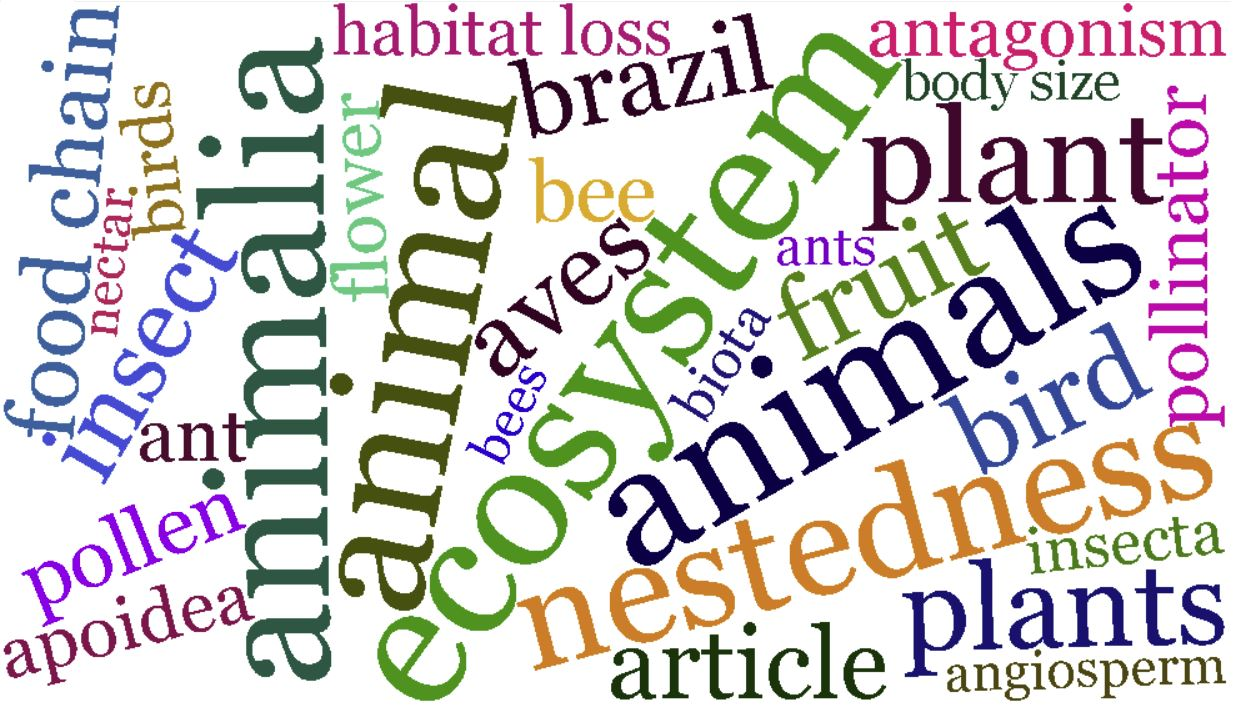
\includegraphics{WordCloud.JPG}
\caption{Nube de palabras}
\end{figure}

\hypertarget{dinuxe1micas-de-las-palabras.}{%
\subsubsection{Dinámicas de las
palabras.}\label{dinuxe1micas-de-las-palabras.}}

En la pestaña \texttt{Documents\textgreater{}Word\ Dynamics} podemos
encontrar un gráfico de ocurrencia acumulada de las palabras a lo largo
del tiempo en nuestro conjunto de artículos.

\begin{figure}
\centering
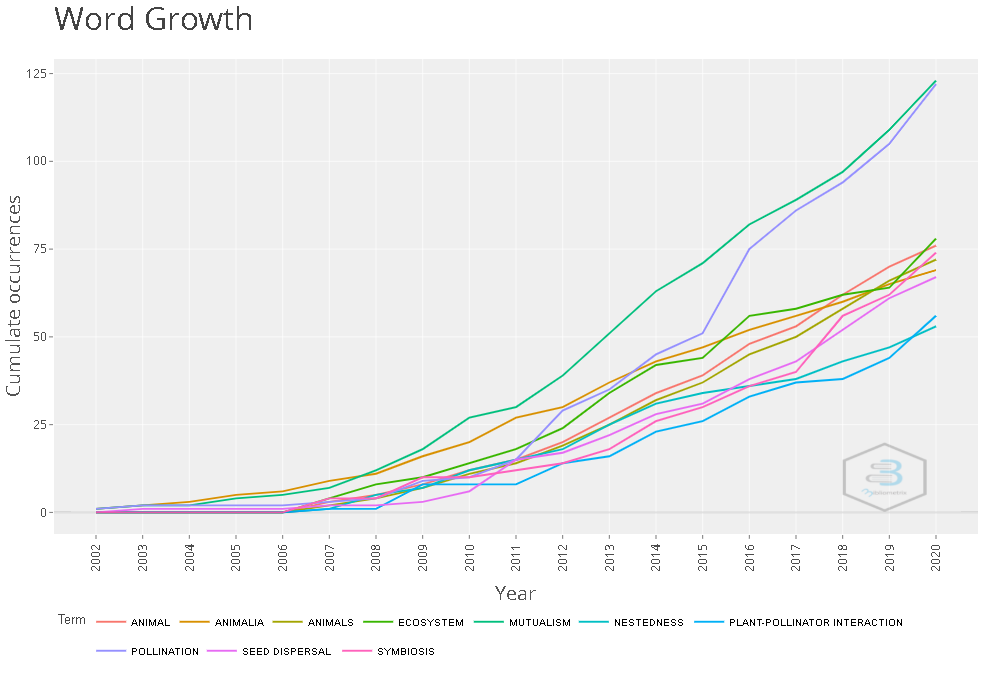
\includegraphics{WordGrowth.png}
\caption{Diagrama de la dinámica de las palabras}
\end{figure}

Podemos observar que los dos temas mas productivos son el mutualismo y
la polinización. Le sigue ecosistemas, animales, simbiosis y dispersion
de semillas. Por ultimo tenemos interaccion planta polinizador y
anidamiento. Todos estos son los conceptos de moda sobre los que puede
ser interesante investigar.

\hypertarget{tuxe9rminos-de-moda.}{%
\subsubsection{Términos de moda.}\label{tuxe9rminos-de-moda.}}

En la pestaña \texttt{Documents\textgreater{}Trend\ Topics} podemos
generar un diagrama con los terminos de moda, en qué momento aparecen y
cuando desaparece, con una serie de burbujas asociadas que describen el
momento en el que mas aparecen y con qué frecuencia, siendo más grandes
cuanto más veces aparecieran en ese marco temporal.

\begin{figure}
\centering
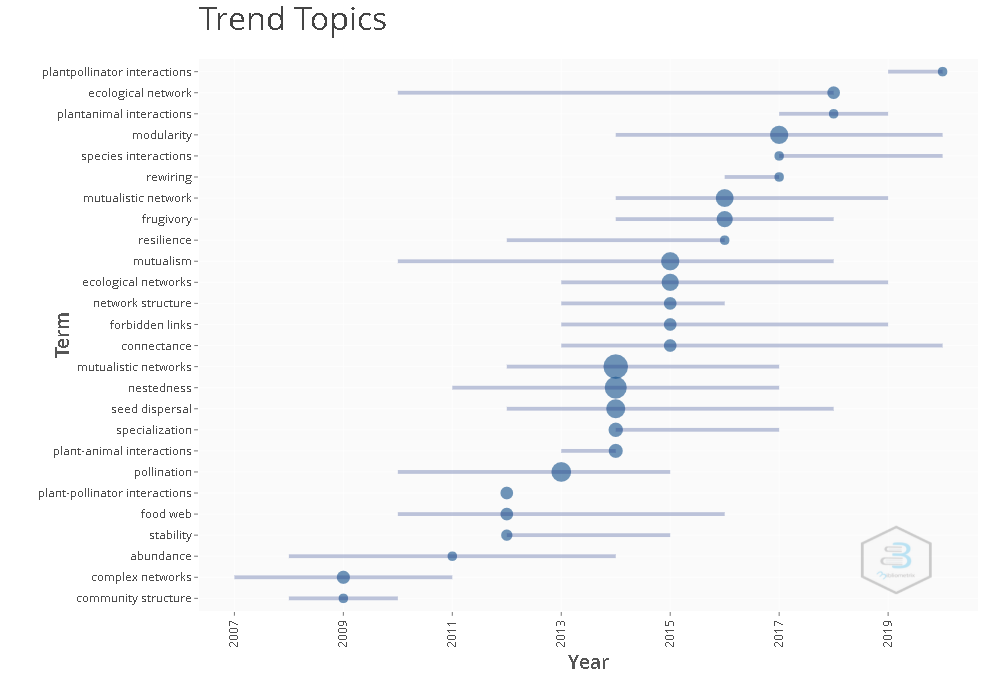
\includegraphics{TrendTopics.png}
\caption{Diagrama de los términos de moda}
\end{figure}

Podemos observar que:

\begin{itemize}
\tightlist
\item
  Los temas iniciales del campo de estudio tienen relación con el
  estudio de redes complejas y redes alimentarias entre 2009 y 2012.
\item
  Las interacciones planta polinizador son un tema común a lo largo de
  todo el marco temporal.
\item
  Las interacciones entre plantas y frugívoros son un tema frecuente
  entre 2014 y 2016.
\item
  Todo el marco temporal está salpicado de temas relacionados con las
  redes, como el anidamiento, la conectancia, el recableado etc.
\end{itemize}

\hypertarget{estructura-conceptual.}{%
\subsection{Estructura conceptual.}\label{estructura-conceptual.}}

\hypertarget{anuxe1lisis-de-la-red.}{%
\subsubsection{Análisis de la red.}\label{anuxe1lisis-de-la-red.}}

El análisis de la red podemos realizarlo principalmente fijándonos en
dos tipos de análisis, el mapa temático y la evolución temática. Para
observar el mapa temático podemos acceder a
\texttt{Conceptual\ Srtucture\textgreater{}Thematic\ Map}. En la primera
pestaña \texttt{Map} podemos observar un mapa de Gallons con los
principales agrupamientos de las palabras de nuestro conjunto
bibliográfico. Se ha cambiado el análisis a 2000 palabras para obtener
una representación con más grupos. Encontramos dos grupos básicos de
temas:

\begin{itemize}
\tightlist
\item
  Temas básicos:

  \begin{itemize}
  \tightlist
  \item
    Animalia, seed dispersal, aves. Tema relacionado con la dispersión
    de semillas y los animales relacionados.
  \item
    Mutualism, nestedness, comunity structure. Tema relacionado con el
    mutualismo, la estructura anidada de las comunidades.
  \item
    Polination, plant-polinator interaction, biodiversitiy. Tema
    relacionado con la polinización y su papel en la biodiversidad.
  \end{itemize}
\item
  Temas de nicho:

  \begin{itemize}
  \tightlist
  \item
    Dos temas relacionados con la extinción (Extintion, ant,
    demograpghy) y (Temporal variation, extinction risk, resource
    availability)
  \item
    Abundance, body size, antropogenic effect. Tema relacionado con los
    ecosistemas y el efecto del ser humano en ellos.
  \item
    Cohort analysis.
  \end{itemize}
\end{itemize}

\begin{figure}
\centering
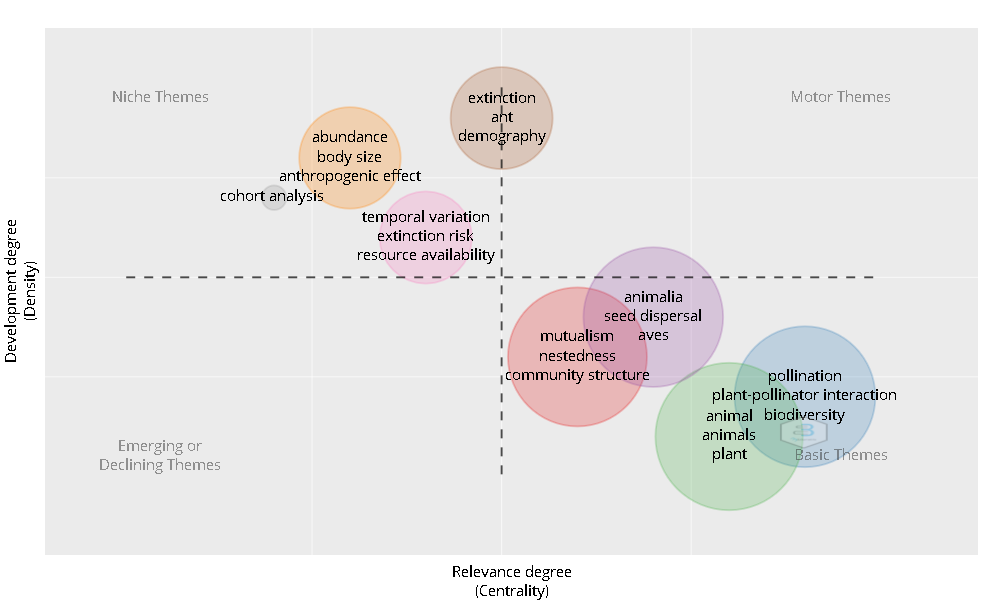
\includegraphics{ThematicMap.png}
\caption{Mapa temático}
\end{figure}

Cuando pasamos a la representación de red podemos observar estos mismos
grupos pero en forma de red. Los colores se corresponden con los mismos
grupos del mapa de Gallons. Aunque la imagen es atractiva, la
información mas relevante se puede sacar del mapa bidimensional que es
una representación de como son las interacciones en esta red. Los temas
básicos (rojo, morado, azul y verde) son los temas que mas se
interconectan con otros grupos, mientras que las interconexiones entre
los nodos del mismo grupo son bajas. Se trata de temas básicos y
transversales. Los temas de nicho (rosa, naranja, marrón y gris)
presentan mas interconexiones entre ellos que con otros grupos. Hacia la
periferia podemos encontrar pequeñas agrupaciones pero es dificil
encontrar un patrón claro dado lo intrincada que es la red. El grupo
perfiérico morado de la zona inferior se corresponde con palabras de
especies de plantas, todas ellas interconectando con fungi. Dado el tema
de las redes mutualistas y las interacciones mutualistas que se dan
entre hongos y plantas, es posible que tengamos artículos sobre
micorrizas. El resto es demasiado intrincado y es mejor sacar
conclusiones a partir del mapa temático.

\begin{figure}
\centering
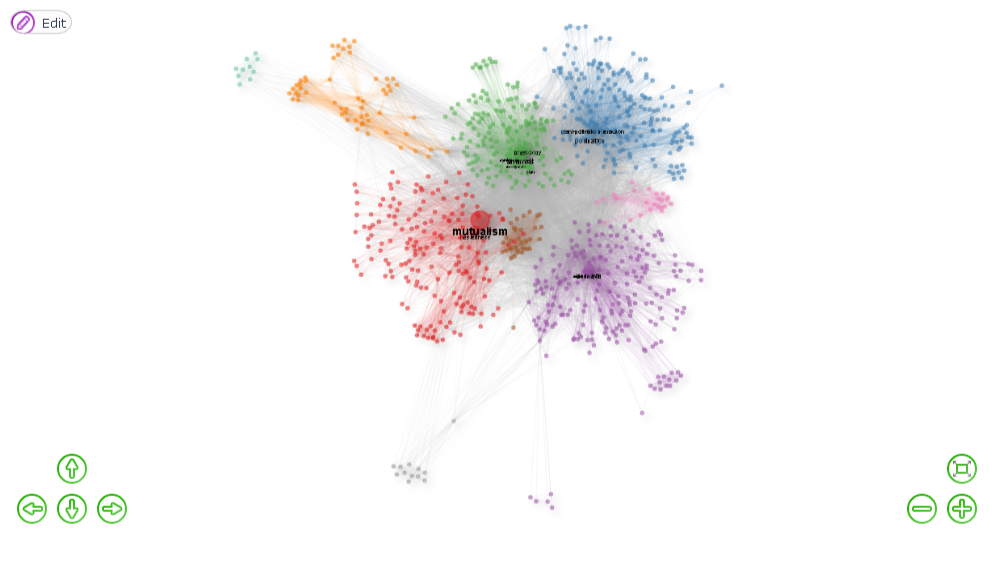
\includegraphics{networkThematicMap.png}
\caption{Red del mapa temático}
\end{figure}

Otro análisis que permite Biblioshiny es el de la evolución temática. La
base es la misma que la del mapa temático, pero aquí podemos restringir
el análisis a un marco temporal restringido, formando lo que denomina
\emph{slices} o cortes. Esto puede ser interesante porque podemos ver
como los temas van evolucionando dentro del mapa temático, es decir,
estamos añadiendo la dimension temporal a nuestro análisis. Para ello
accedemos a la pestaña
\texttt{Conceptual\ Structure\textgreater{}Thematic\ Evolution}, ponemos
el número de palabras en 2000 y añadimos 3 cortes. Colocamos los Cutting
Years aproximadamente equidistantes para obtenener marcos temporales de
la misma longitud. Elejimos los años 2006, 2010, y 2014.

\begin{itemize}
\tightlist
\item
  TimeSlice 1. Un tema neutro en centralidad y densidad que es
  polinización. Animalia como un tema transversal o basico.
\end{itemize}

\begin{figure}
\centering
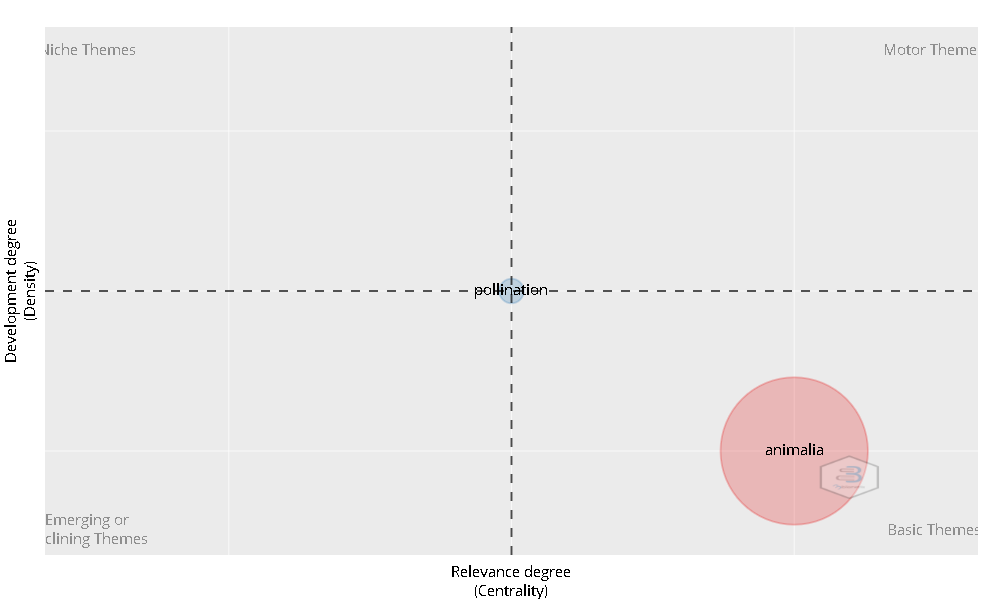
\includegraphics{ThematicEvolutionSlice1.png}
\caption{Evolución temática. Primer corte.}
\end{figure}

\begin{itemize}
\tightlist
\item
  TimeSlice 2. Aparece plant-polinator interaction como un tema muy
  fructifero y relacionado. Probablemente de lugar a otros temas en el
  futuro. La diversidad de especies aparece como un tema de nicho poco
  interrelacionado. El mutualismo aparece como un tema predominantemente
  poco conectado tanto a nivel interno como externo. Esto puede ser
  indicativo de que es un tema emergente o en declive, esto depende de
  lo que observemos en futuros cortes.
\end{itemize}

\begin{figure}
\centering
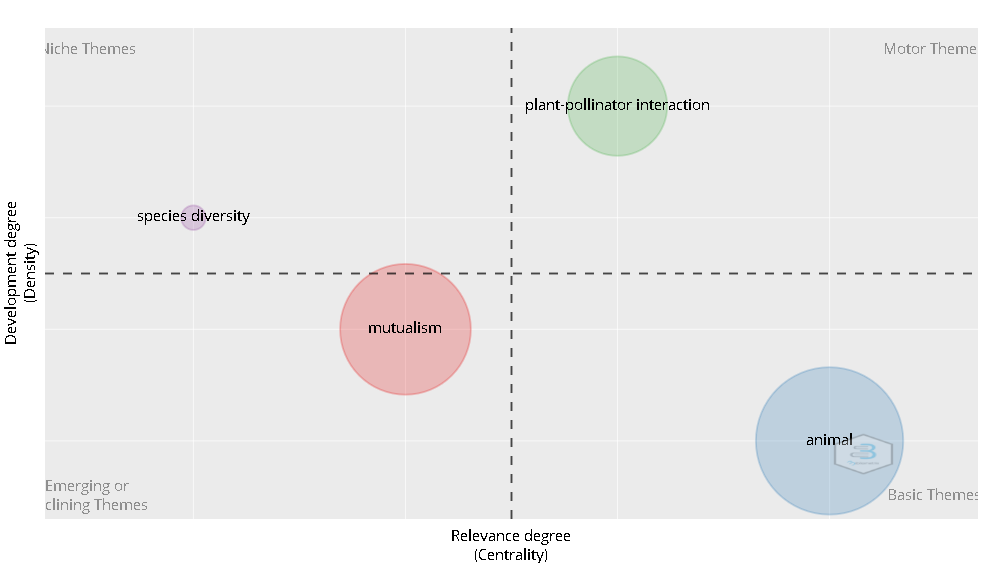
\includegraphics{ThematicEvolutionSlice2.png}
\caption{Evolución temática. Segundo corte.}
\end{figure}

\begin{itemize}
\tightlist
\item
  TimeSlice 3. El mutualismo ha derivado a un tema con centralidad y
  densidad medias, por lo que se trataba anteriormente de un tema
  emergente. Introduced species aparece como tema emergente o en
  declive. Animalia y nestednees aparecen como temas muy fructiferos e
  importantes.
\end{itemize}

\begin{figure}
\centering
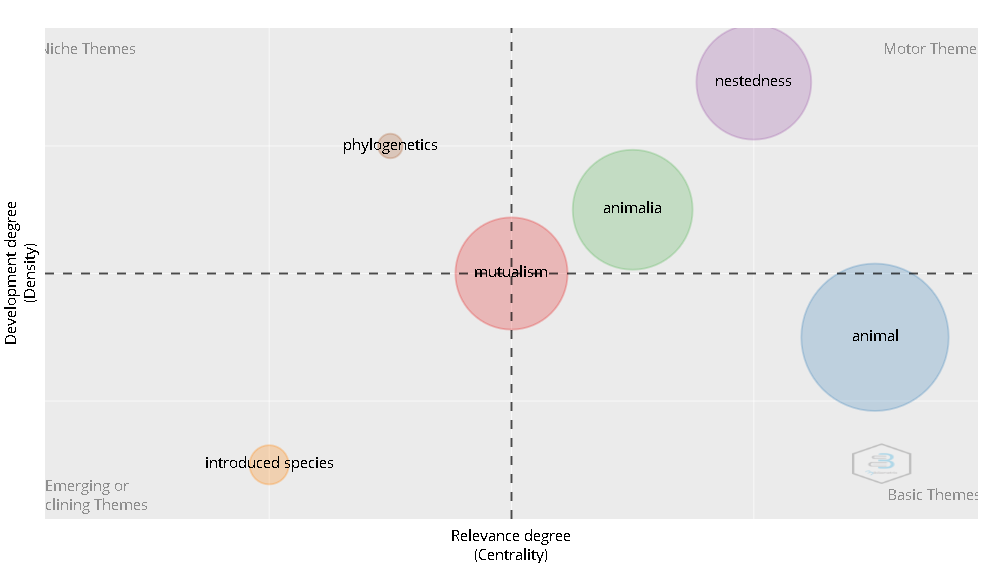
\includegraphics{ThematicEvolutionSlice3.png}
\caption{Evolución temática. Tercer corte.}
\end{figure}

\begin{itemize}
\tightlist
\item
  TimeSlice 4. Ahora el tema motor es el análisis de red. Los temas
  basicos ahora es el mutualismo que antes aparecia como tema motor, la
  polinización y los animales. Aparecen varios temas de nicho como la
  abundancia o los hongos. Las especies introducidas eran un tema
  emergente que derivo en un tema de nicho. Evolución aparece como un
  tema poco conectado dentro de su propia red pero mas interconectado
  con otros temas.
\end{itemize}

\begin{figure}
\centering
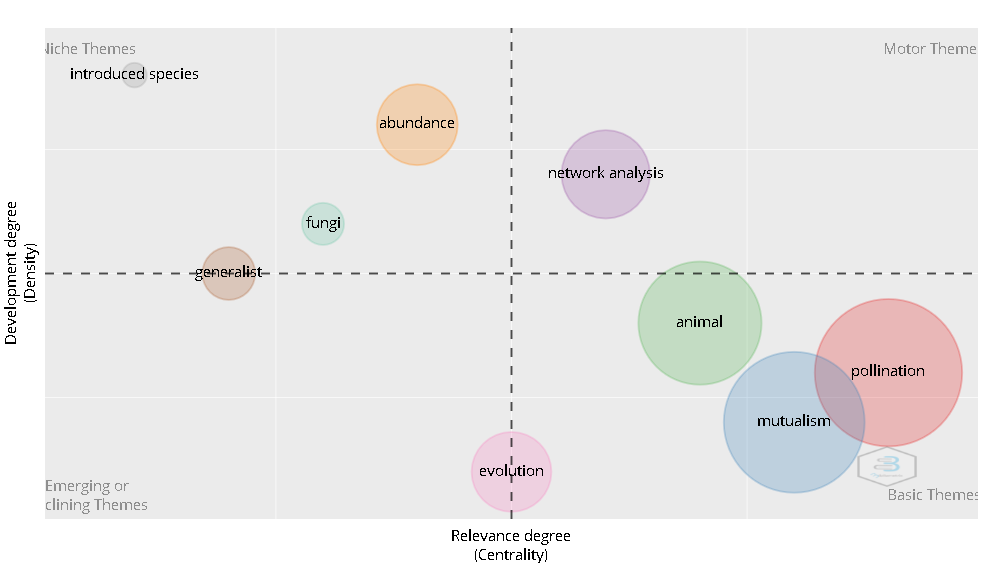
\includegraphics{ThematicEvolutionSlice4.png}
\caption{Evolución temática. Cuarto corte.}
\end{figure}

En la pestaña thematic evolution podemos encontrar una representación de
esto que hemos comentado pero en columnas con los temas que aparecen y
con lineas de flujo que conectan los temas que derivan unos de otros.

\begin{figure}
\centering
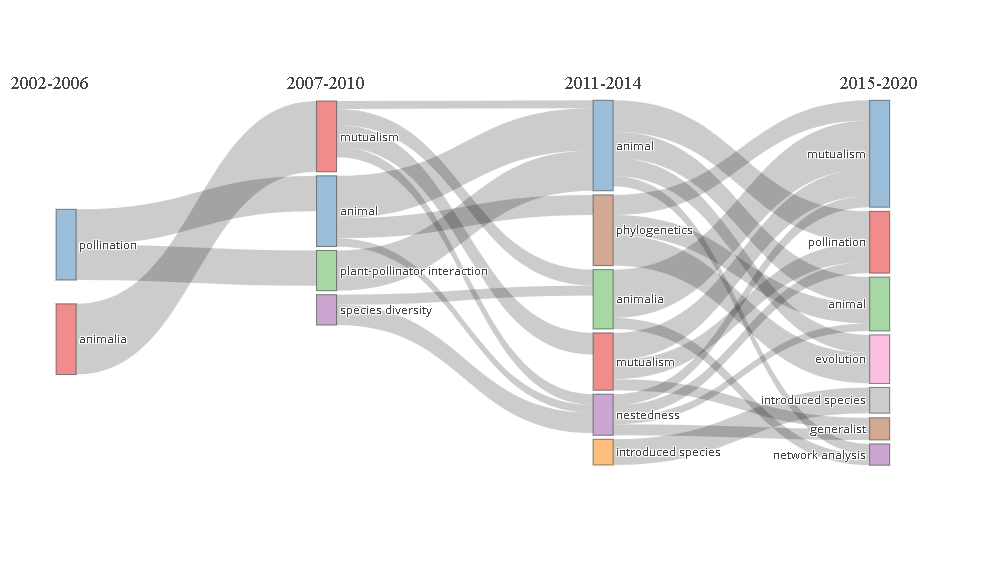
\includegraphics{ThematicEvolutionTotalView.png}
\caption{Visión completa de la evolución temática}
\end{figure}

\hypertarget{anuxe1lisis-factorial.}{%
\subsubsection{Análisis factorial.}\label{anuxe1lisis-factorial.}}

En la pestaña
\texttt{Conceptual\ Structure\textgreater{}Factorial\ Analysis} podemos
realizar un análisis factorial de distintos elementos como:

\begin{itemize}
\tightlist
\item
  Palabras: medimos la similitud en función de la cantidad de veces que
  dichas palabras aparecen juntas en un artículo.
\item
  Artículos: medimos su similitud en función de su nivel de influencia o
  el número de citas.
\end{itemize}

Podemos elegir entre un análisis de correspondencia o un análsisis de
correspondencia múltiple, en nuestro caso es el segundo método el que
ofrece una gráfica más representativa de la variabilidad de los datos
(64.62\%).

\begin{figure}
\centering
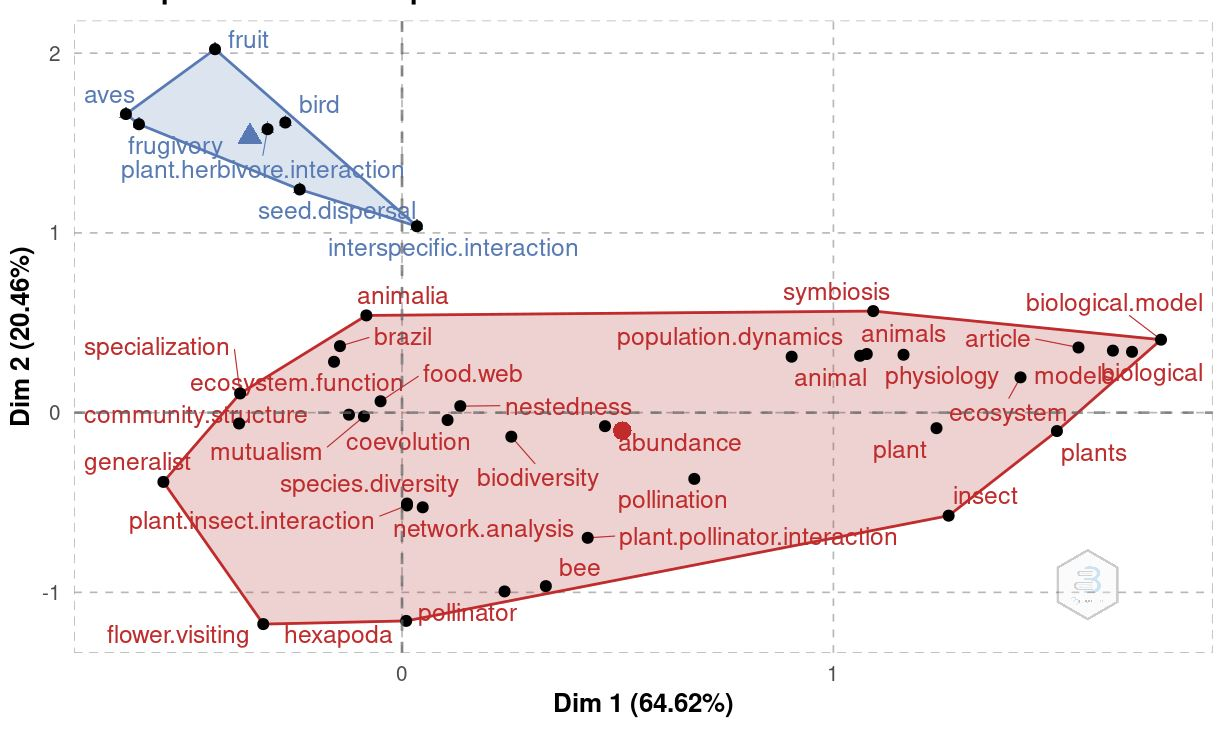
\includegraphics{MapaAnalisisFactorial.JPG}
\caption{Mapa del análisis factorial de palabras}
\end{figure}

Podemos observar dos agrupamientos diferneciados. En azul, conceptos
relacionados con las interacciones entre plantas y animales en las que
se produce algún tipo de herbivoría, como la frugivoría o la dispersión
de semillas. Encontramos los conceptos fruit, sedd.dispersal, bird, etc.
En rojo encontramos conceptos relacionados con la polinización y el
estudio de redes. Podemos discrepar de la cantidad de agrupaciones
realizadas por biblioshiny. En este mapa conceptual, en el grupo de
abajo parece que podemos dividirlo en otro dos grupos, uno a la derecha
y otro a la izquierda. Por defecto el número de agrupamientos vienen en
Auto, pero si lo cambiamos a tres nos ofrece unas agrupaciones con más
sentido.

\begin{figure}
\centering
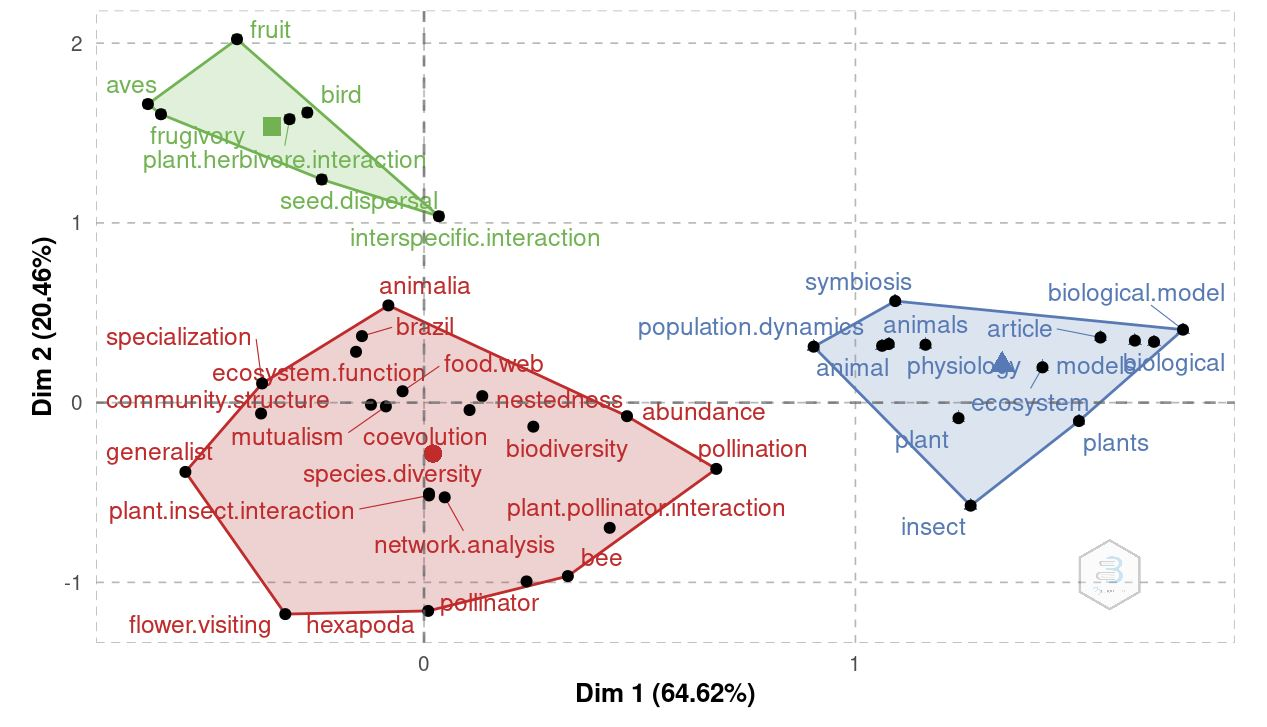
\includegraphics{MapaAnalisisFactorial3Grupos.JPG}
\caption{Mapa del análisis factorial de palabras con 3 agrupaciones}
\end{figure}

Con este nuevo análisis encontramos un nuevo grupo con conceptos
relacionados con la simbiosis, los animales, las plantas y los insectos.
Podemos representar esta misma información pero en forma de dendrograma.

\begin{figure}
\centering
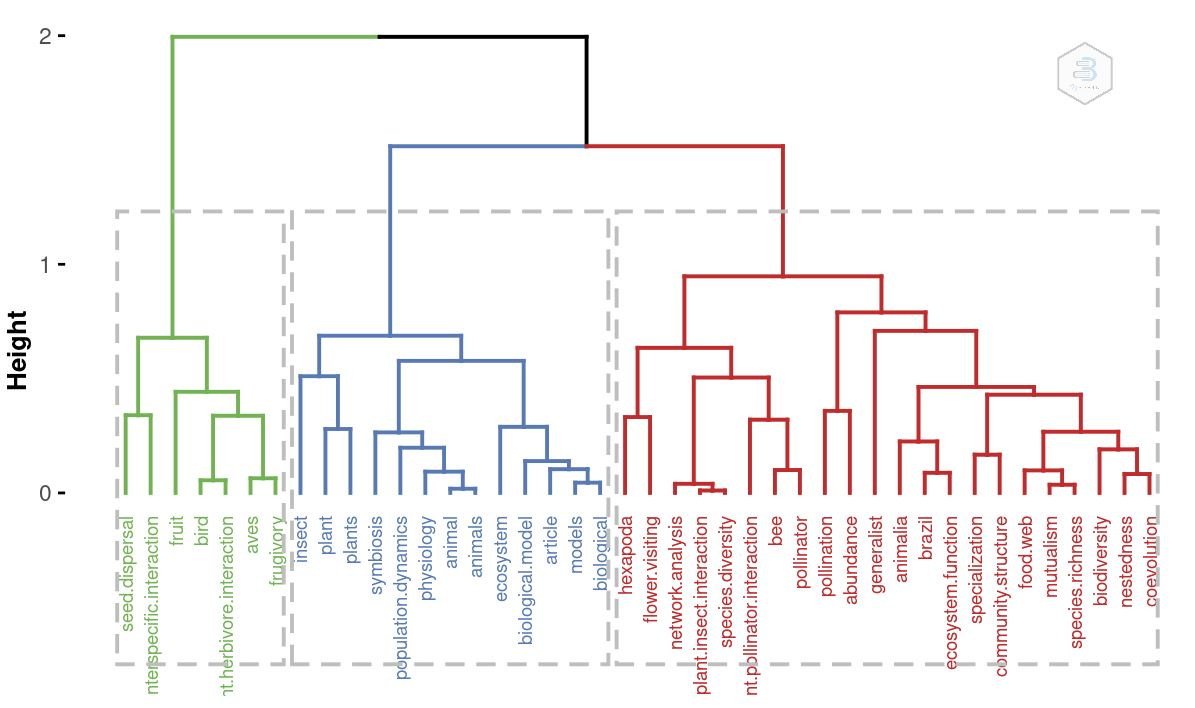
\includegraphics{DendrogramaAnalisisFactorial.JPG}
\caption{Dendrograma del análisis factorial de palabras}
\end{figure}

El dendrograma ofrece esencialmente la misma información que el mapa.
Podemos generar un mapa conceptual de los artículos mas contributivos o
los mas citados.

\begin{figure}
\centering
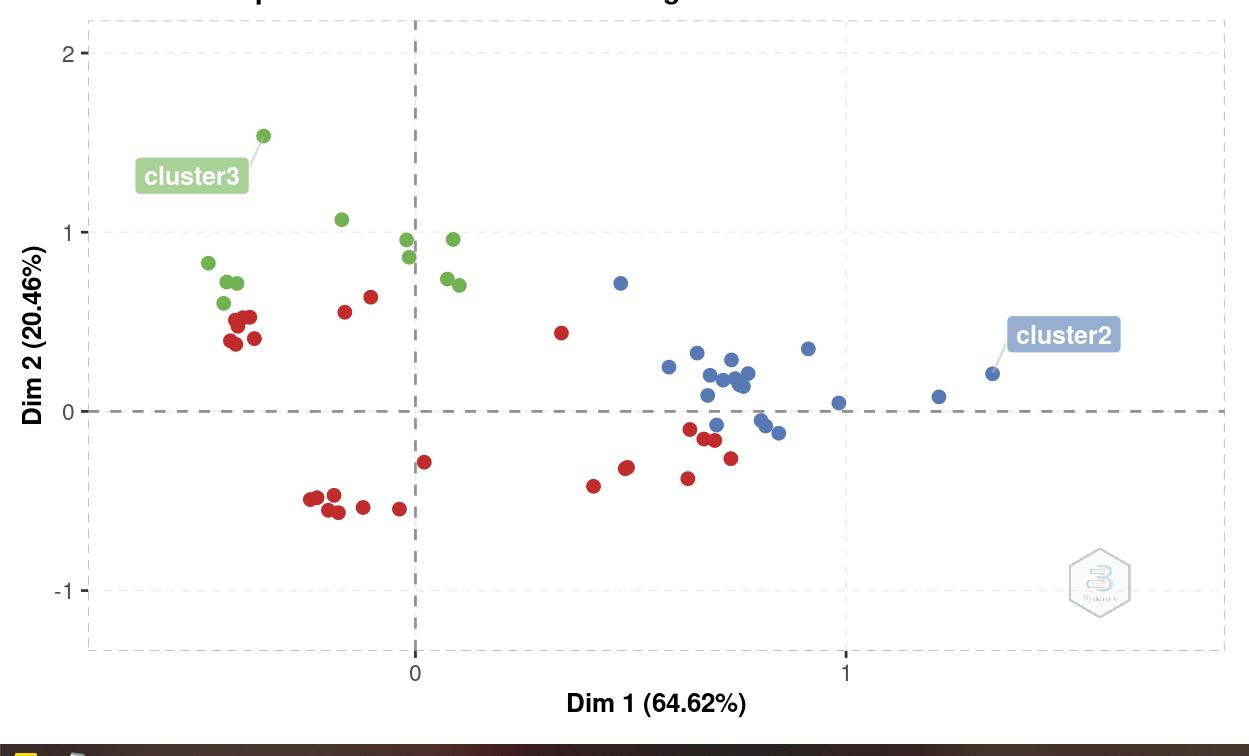
\includegraphics{MapaAnalisisFactorialArticulosMasContributivos.JPG}
\caption{Mapa del análisis factorial de artículos mas contributivos con
3 agrupaciones}
\end{figure}

Para identificar los artículos es conveniente acceder a la tabla de la
pestaña \texttt{Articles\ By\ Cluster}.

\hypertarget{estructura-intelectual.}{%
\subsection{Estructura intelectual.}\label{estructura-intelectual.}}

\hypertarget{red-de-co-citacion.}{%
\subsubsection{Red de co-citacion.}\label{red-de-co-citacion.}}

En la pestaña
\texttt{Intelectual\ Structure\textgreater{}Co-citation\ Network}
podemos generar redes de co-citación de artículos, autores y papers.
Pondremos como ejemplo una red de co-citación de autores, que puede
darnos información sobre qué grupos de autores interactuan mas entre
ellos.

\begin{figure}
\centering
\includegraphics{RedDeCocitaciónAutores.png}
\caption{Red de co-citación de los autores}
\end{figure}

Podemos observar que existen 4 autores que interactúan mucho entre sí:
Bascompte, Jordano, Vazquez y Olesen. Alrededor de ellos encontramos un
conjunto de autores que presenta muchas conexiones con estos autores.
Encontramos otrso dos grupos, uno liderado por Memmot y otro por
Guimares y Thompson. Sin embargo, estos otros dos grupos parecen
presentar menos conexiones entre ellos que con el grupo de Bascompte,
además sus autores son menos productivos.

\hypertarget{historiografuxeda.}{%
\subsubsection{Historiografía.}\label{historiografuxeda.}}

La historiografía uno los artículos como en la red de co-citación pero
además los ordena en función de su fecha de publicación. Esto nos
permite seguir la evolución de los temas. En la pestaá
\texttt{Intellectual\ Structure\textgreater{}Historiograph} podemos
generar una historiografía de nuestra muestra bibliográfica. Recomiendo
bajar el número de nodos a 10 para hacer un diagrama más legible.
Tambien es interesante cambiar la etiqueta de los nodos por el titulo
del documento, ya que una rápida lectura de los titulos puede ayudarnos
a inferir superficialmente la evolución de los temas.

\begin{figure}
\centering
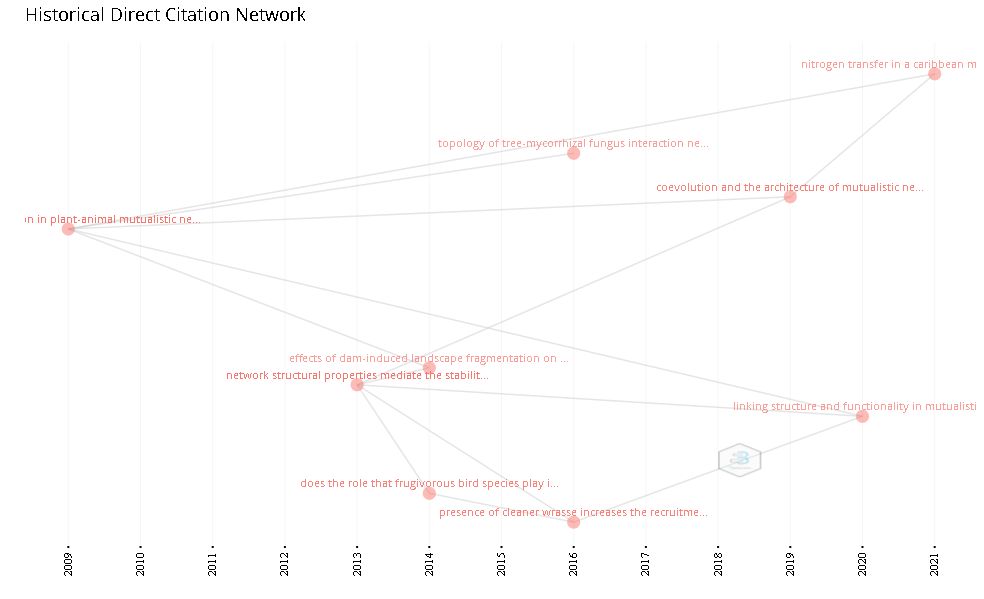
\includegraphics{Historiografia.png}
\caption{Historiografía}
\end{figure}

El primer artículo del que surgen muchos otros habla sobre la
distribución del grado en redes mutualistas planta polinizador. Esto
parede derivar en multitud de temas, entre los que tenemos:

\begin{itemize}
\tightlist
\item
  A)Efecto de la fragmentación del habitat en las redes hormiga-planta
  del amazonas.
\item
  B)Uniendo funcionalidad y estructura. El papel de los frugivoros.
\item
  C)Coevolución y arquitectura de redes mutualistas.
\item
  D)Topología de las redes planta-micorriza.
\item
  E)Transferencia de nitrógeno en redes mutualistas caribeñas.
\end{itemize}

El artículo A) deriva a su vez en otro artículo que habla sobre la
estructura de las redes y su papel en la estabilidad de las comunidades
(A1). A1 deriva a su vez en un grupo de artículos bien interconectado:

\begin{itemize}
\item
  A1a)El role de las aves frugivoras en las redes de dispersión tiene un
  papel en la divergencia evolutiva?
\item
  A1b)La presencia de peces limiadores aumenta la presencia del pez
  damisela en arrecifes de coral. Curiosamente este artículo no parece
  relacionarse con las redes mutualistas, pero dado que parece derivar
  de este tema puede ser interesante echarle un vistazo para ver si
  aporte al campo de estudio o se nos ha colado en el análisis.
\item
  \begin{enumerate}
  \def\labelenumi{\Alph{enumi})}
  \setcounter{enumi}{1}
  \tightlist
  \item
    El artículo B tambien conecta con el A1.
  \end{enumerate}
\end{itemize}

\hypertarget{estructura-social.}{%
\subsection{Estructura social.}\label{estructura-social.}}

\hypertarget{red-de-colaboraciuxf3n.}{%
\subsubsection{Red de colaboración.}\label{red-de-colaboraciuxf3n.}}

En la pestaña
\texttt{Social\ Structure\textgreater{}Collaboration\ Network} podemos
generar una red de colaboración. A diferencia de las redes de
co-citación, las redes colaboración unen nodos (generalmente autores)
cuando presentan artículos donde ambos figuran como co-autores.

\begin{figure}
\centering
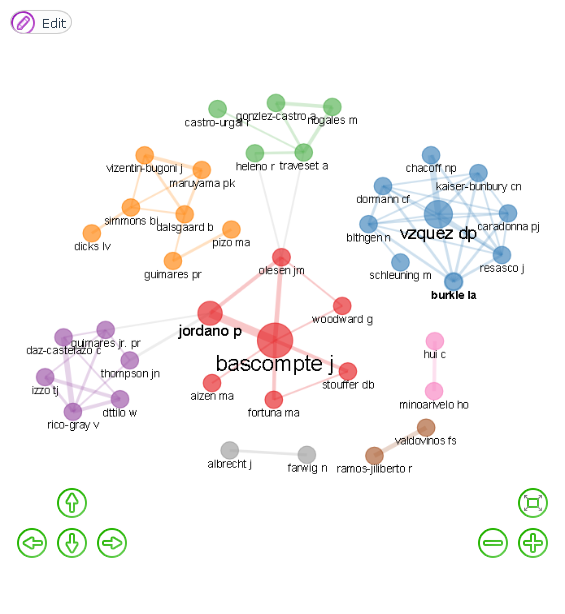
\includegraphics{RedDeColaboracion.png}
\caption{Red de colaboración}
\end{figure}

La red ha sido alterada para mostrar los conjuntos mas cercanos entre
sí. Parece ser que las redes de colaboración presentan mayor tendencia a
fragmentarse, probablemente porque es más sencillo citar a otro autor
que colaborar con él. Las colaboraciones acaban siendo más restringidas
y formando redes de autores separadas que tiene a colbaorar entre sí.
Los dos grupos mas grandes son el de Bascompte y Vazquez. Bascompte
tienen menos nodos pero mas grandes, son pocos autores pero más
contributivos, mientras que ocurre al contrario con el de Vazquez. El
grupo de Bascompte sí presenta interacciones con otros grupos como el de
Thompson o el de Gonzalez Castro.

\hypertarget{mapa-de-colaboraciuxf3n.}{%
\subsubsection{Mapa de colaboración.}\label{mapa-de-colaboraciuxf3n.}}

Aunque la red de colaboración permite generar una red de colaboraciones
entre los paises de los autores es preferible acceder a
\texttt{Social\ Structure\textgreater{}Collaboration\ Map}. Esta
herramienta de Biblioshiny permite generar un Mapa Mundi donde los
paises aparecen en tonos de azul en función de la cantidad de artículos
producidos y aparecen lineas que unen los paises que han contribuido,
mostrando en su grosor la cantidad de colaboraciones. He aumentado el
número minimo de enlaces a 6 para hacer el mapa más legible.

\begin{figure}
\centering
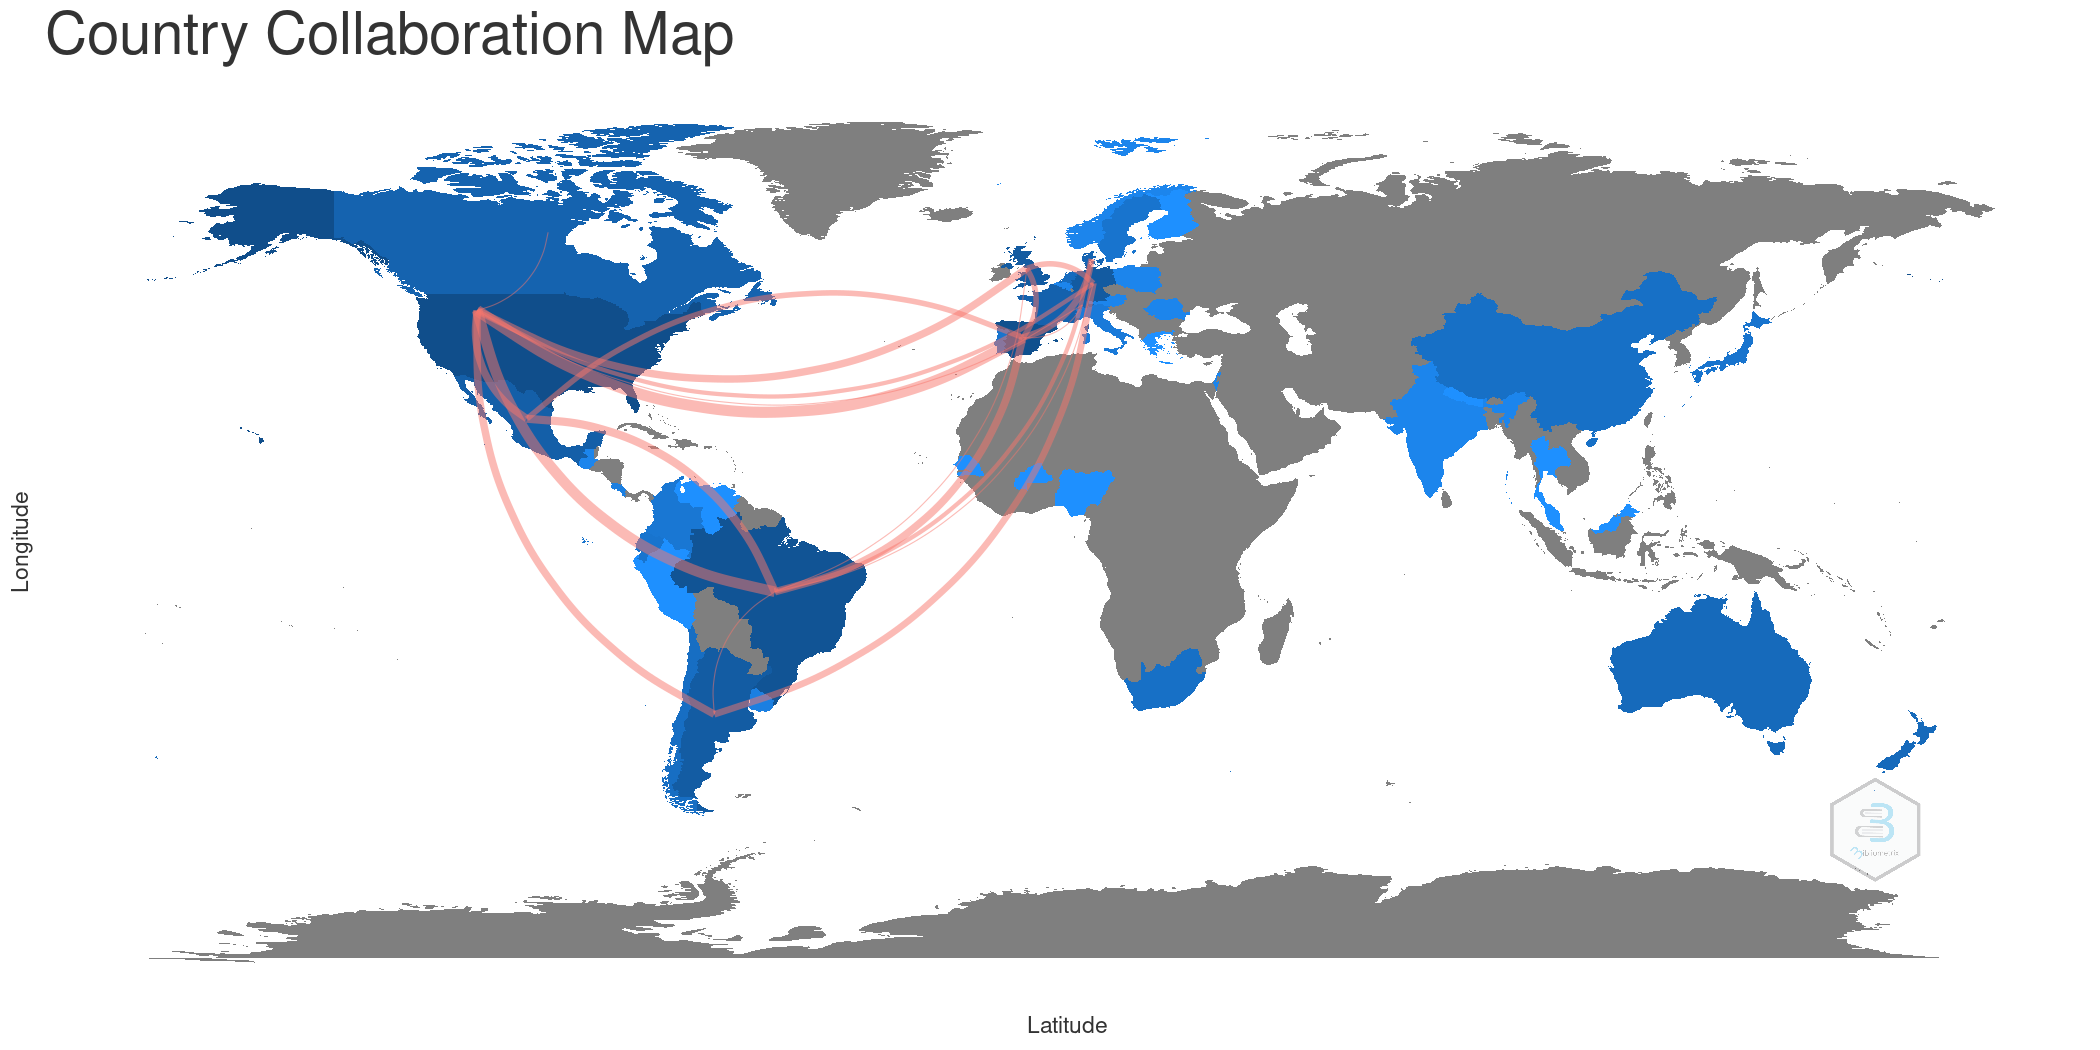
\includegraphics{CountryCollaborationMap-2022-01-05.png}
\caption{Mapa de colaboraciones}
\end{figure}

Las 10 colaboraciones más frecuentes se pueden observar en la siguiente
tabla.

\begin{longtable}[]{@{}lll@{}}
\toprule
biblioshiny for bibliometrix & & \\
\midrule
\endhead
From & To & Frequency \\
USA & SPAIN & 16 \\
USA & BRAZIL & 15 \\
BRAZIL & MEXICO & 11 \\
BRAZIL & SPAIN & 10 \\
USA & ARGENTINA & 10 \\
USA & MEXICO & 10 \\
USA & UNITED KINGDOM & 10 \\
ARGENTINA & GERMANY & 9 \\
SPAIN & DENMARK & 9 \\
GERMANY & UNITED KINGDOM & 8 \\
\bottomrule
\end{longtable}

\hypertarget{anexos.}{%
\section{Anexos.}\label{anexos.}}

\hypertarget{tuxe9rminos-utilizados-en-la-informaciuxf3n-principal.}{%
\subsection{Términos utilizados en la información
principal.}\label{tuxe9rminos-utilizados-en-la-informaciuxf3n-principal.}}

\begin{itemize}
\tightlist
\item
  \textbf{Timespan}: Año del primer y el último artículo
  publicado.\footnote{Algunos artículos pueden presentarse borradores
    pendientes de revisión, con fechas de publicación a futuro. Esto
    explica la existencia de artículos a fecha de 2022, cuando la
    muestra bibliográfica se descargó en 2021.}
\end{itemize}

\begin{itemize}
\tightlist
\item
  \textbf{Sources (Journals, Books, etc)}: Fuentes de las que provienen
  los documentos, revistas, libros etc.
\item
  \textbf{Documents}:total de documentos\\
\item
  \textbf{Average years from publication}: Promedio de años entre la
  publicación de un documento y sus primeras citas.\\
\item
  \textbf{Average citations per documents}: Promedio de citas por
  documento.
\end{itemize}

\[
\text{Average citations per documents}=\frac{\text{total de citas}}{\text{total de documentos}}
\]

\begin{itemize}
\tightlist
\item
  \textbf{Average citations per year per doc}: Promedio de citas por año
  y por documento.
\end{itemize}

\[
\text{Average citations per year per doc}=\frac{\text{total de citas}}{\text{total de documentos}*\text{duracion en años del marco temporal}}
\]

\begin{itemize}
\tightlist
\item
  \textbf{References}: Total de citas en toda la muestra.\\
\item
  \textbf{article}: Total de artículos.\\
\item
  \textbf{book}: Total de libros.\\
\item
  \textbf{book chapter}: Total de capítulos de libros.\\
\item
  \textbf{editorial}: Total de editoriales.\\
\item
  \textbf{letter}: Total de cartas.
\item
  \textbf{note}: Total de notas.\\
\item
  \textbf{review} Total de revisiones.\\
\item
  \textbf{short survey}: Total de estudios breves.\\
\item
  \textbf{Keywords Plus (ID)}: Total de palabras clave plus. Las
  palabras clave plus son palabras clave generadas automáticamente por
  la base de datos en cuestión a partir de las palabras más comunes que
  aparecen en los títulos de los artículos citados.
\item
  \textbf{Author's Keywords (DE)}: Total de palabras clave de autores.
  Las palabras clave de autores son las palabras clave que son indexadas
  manualmente por los propios autores de los artículos.
\item
  \textbf{Authors}: Total de autores.\\
\item
  \textbf{Author Appearances}: Total de veces que los autores aparecen
  como tal en los documentos.\\
\item
  \textbf{Authors of single-authored documents}: Total de autores que
  aparecen en documentos con un solo autor.
\item
  \textbf{Authors of multi-authored documents} Total de autores que
  aparecen en documentos con múltiples autores. -
  \textbf{Single-authored documents} Total de documentos con un solo
  autor.\\
\item
  \textbf{Documents per Author}: Documentos por autor.
\end{itemize}

\[
\text{Documents per Author}=\frac{\text{total de documetnos}}{\text{total de autores}}
\]

\begin{itemize}
\tightlist
\item
  \textbf{Authors per Document}: Autores por documento.
\end{itemize}

\[
\text{Authors per Document}=\frac{\text{total de autores}}{\text{total de documentos}}
\]

\begin{itemize}
\tightlist
\item
  \textbf{Co-Authors per Documents}: Coautores por documento.
\end{itemize}

\[
\text{Co-Authors per Documents}=\frac{\text{total de coautores}}{\text{total de documentos}}
\]

\begin{itemize}
\tightlist
\item
  Collaboration Index: Índice de colaboración.
\end{itemize}

\[
\text{Collaboration Index}=\frac{\text{total de coautores}}{\text{total de documentos con coautoría}}
\]

\hypertarget{ratio-de-crecimiento-anual-compuesto.}{%
\subsection{Ratio de crecimiento anual
compuesto.}\label{ratio-de-crecimiento-anual-compuesto.}}

El cálculo del ratio de crecimiento en la producción científica anual se
realiza a través de la ecuación para el cálculo del ratio de crecimiento
anual compuesto(\(CAGR\)):

\[
CAGR(t_0, t_n)=\left({\frac{V(t_n)}{V(t_0)}}\right)^{\frac{1}{t_n-t_0}}-1
\]

En nuestro caso, \(V(t_n)\) es la cantidad de artículos en el último
año, \(V(t_0)\) es la cantidad de artículos en el año inicial y \(t_n\)
y \(t_0\) los años finales e inicial de nuestro marco temporal
respectivamente. \(CAGR\) puede tomar valores positivos, negativos o 0,
para lo cual:

\[
CAGR>0; crecimiento
\]

\[
CAGR=0; estable
\]

\[
CAGR<0; decrecimiento
\]

\hypertarget{ley-de-bradford.-1}{%
\subsection{Ley de bradford.}\label{ley-de-bradford.-1}}

La siguiente explicación es una adaptación de las páginas 95-8 de Bellis
(2009). La ley de bradford propone que si ordenamos las revistas en
orden decreciente de procutividad (nº de artículos publicados)
observaremos que existe un ``núcleo'' de revistas que acumulan la mayor
parte de los artículos de nuestro tema de estudio, mientras que el resto
de los artículos se diespersan entre un número mucho mayor de revistas
menos productivas. Cuando Samuel Bradford estudiaba un caso práctico con
bibliografía sobre geofísica observo que:

\begin{enumerate}
\def\labelenumi{\arabic{enumi}.}
\tightlist
\item
  Existia un grupo de 9 revistas que acumulaban en total 429 artículos.
\item
  Un segundo grupo de 59 revistas que acumulanan 499 artículos y
\item
  Un tercer grupo de 258 revistas que acumulaban 404 artículos.
\end{enumerate}

Los tres grupos presentan un número similar de artículos a sus espaldas,
pero el segundo y el tercer grupo presentan un número de revistas mucho
mayor, lo que provoca que esos artículos se encuentren mas dispersos. El
número de revistas de cada grupo puede ser expresado como una proporción
del primer grupo, es decir 9:

\begin{enumerate}
\def\labelenumi{\arabic{enumi}.}
\tightlist
\item
  \(9\) revistas del primer grupo.
\item
  \(9*5\) revistas del segundo grupo (\(9*5=45\) aproximadamente 59).
\item
  \(9*5*5=9*5^2\) revistas del tercer grupo (\(9*5^2=225\)
  aproximadamente 258).
\end{enumerate}

Así, las proporciones entre los grupos podrían excribirse como:

\[
9:9*5:9*5^2
\]

Podemos escribir este caso partícular como una ley general para un
conjunto de artículos de una muestra bibliográfica dividiendo cada
elemento por \(9\) y tomando el factor \(5\) como cualquier número
\(m\), ya que no necesariamente tiene que ser 5. La ecuación queda de la
siguiente manera:

\[
1:m:m^2
\]

La secuencia de proporciones anterior equivale a decir que el grueso de
los artículos sobre un tema determinado se concentra en un pequeño
conjunto de revistas del núcleo y luego se dispersa por otras revistas
hasta tal punto que, si el conjunto de artículos relevantes se subdivide
en grupos o zonas que contienen el mismo número de artículos que el
núcleo, se necesitará un número exponencialmente creciente de revistas
para llenar las zonas sucesivas.

Por lo tanto, la ley de Bradford nos puede dar información relevante
sobre cuáles son las revistas científicas más importantes en nuestro
campo, lo que puede guiar nuestra busqueda bibliográfica y prestar
atrención a dichas fuentes.

\hypertarget{uxedndices-bibliomuxe9tricos.}{%
\subsection{Índices
bibliométricos.}\label{uxedndices-bibliomuxe9tricos.}}

Los índices bibliométricos son números extraídos del procesamiento
estadístico de los datos bibliográficos y que pretenden resumir en un
vistazo alguno de los aspectos de dicha muestra. En relación a la
medición del impacto de los autores, hace tiempo que se quiere encontrar
una especie de índice perfecto y universal que permita medir el impacto
de cualquier autor científico en cualquier disciplina(GÃ!{}`lvez Toro,
2006). La realidad dista mucho de ser tan sencilla ya que el impacto de
un autor es muy dependiente del contexto científico en el que se mueve.
A continuación detallaremos los fundamentos de tres índices que se
pueden calcular con Biblioshiny, el principal es el índice \(h\),
mientras que el \(g\) y el \(m\) pretenden corregir las deibilidades del
primero.

\hypertarget{uxedndice-h.}{%
\subsubsection{\texorpdfstring{Índice
\(h\).}{Índice h.}}\label{uxedndice-h.}}

El índice \(h\) fue propuesto por Hirsch (2005) es un número que
pretende resumir el impacto que tiene un investigador dentro de su campo
de estudio. El número h de un investigador es el número de artículos
publicados por dicho investigador que tienen un número igual o mayor de
citas. Por ejemplo, un investigador puede tener un total de 6 artículos
donde tiene 6 o más citas, por debajo podríamos encontrar tal vez 12
artículos que tienen menos de 12 citas y por lo tanto no puede
utilizarse como índice \(h\). Intuitivamente podemos entender que cuanto
mayor sea el índice \emph{H} mayor será el impacto de dicho autor. Para
hacernos una idea, según el citado artículo de Hirsch (2005), los
premios nobel de física suelen presentar un índice \(h\) de 35-39.

Sin embargo, podrás darte cuenta de que el índice H es propuesto
inicialmente para medir impacto de autores, mientras que biblioshiny
propone estos índices para medir impacto de revistas. Matemáticamente no
existe impedimento, ya que tanto autores como revistas son elementos de
una bibliografía de los que se pueden contar artículos publicados y sus
citaciones.

\hypertarget{uxedndice-g.}{%
\subsubsection{\texorpdfstring{Índice
\(g\).}{Índice g.}}\label{uxedndice-g.}}

Una de las desventajas del índice H es que, así como desprecia aquellos
artículos muy poco citados, lo cual es ventajoso, minusvalora aquellos
artículos que presentan muchísimas citas y que pueden haber sido muy
influyentes en el campo de estudio que estamos analizando. Por ejemplo,
supongamos que un autor tiene un índice \(h\) de 15, esto quiere decir
que tiene un total de 15 artículos que han sido citados al menos 15
veces. Si el autor escribe un artículo que tiene muchísima repercusión y
adquiere muchísimas citas, pongamos 50, el recálculo del índice \(h\) no
nos informará de este impacto, porque este nuevo artículo pasará
directamente a la cima de sus artículos más citados.

Debido a la necesidad de darle más importancia a los artículos que son
muy citados, Egghe (2006) ideó el índice \(g\). El índice \(g\) se
calcula de manera muy similar al índice \(h\), primero se ordenan todos
los artículos desde los más citados a los menos citados. Ahora, en vez
de buscar aquel grupo de \(h\) artículos con \(h\) o más citas, buscamos
aquel grupo de \(h\) artículos que tenga \(h^2\) o más citas, en
adelante \(g\) citas. ¿Qué obtenemos elevando las citas al cuadrado?
Cuando elevas un número pequeño al cuadrado este hace más grande, pero
si elevas un número grande al cuadrado este se hace muchísimo más
grande. Por ejemplo, \(2^2=4\) donde \(4\) es el doble que \(2\), pero
\(100^2=10.000\) donde \(10.000\) es cien veces más que \(100\). Con
esto conseguimos dos cosas interesantes:

\begin{itemize}
\tightlist
\item
  Le damos más valor a los artículos muy citados.
\item
  Ganamos precisión al comparar autores que presentan muchisimas citas.
\end{itemize}

\hypertarget{uxedndice-m.}{%
\subsubsection{\texorpdfstring{Índice
\(m\).}{Índice m.}}\label{uxedndice-m.}}

El índice \(m\) pretende contrarrestar la sobrerrepresentación que
pueden presentar los autores con carreras investigadoras más largas, ya
que el tiempo que lleva un investigador en activo no es tomado en cuenta
por el índice \(h\), lo que puede provocar que los investigadores
noveles acaben infrarrepresentados. Para ello, el índice \(m\) es una
simple derivación del índice \(h\) que consiste en dividir este índice
por la cantidad de años que han pasado desde que el autor publicón su
primero artículo(\(t\)).

\(Índice m=\frac{\text{Índice h}}{t}\)

\hypertarget{frecuencia-fraccionalizada.}{%
\subsection{Frecuencia
fraccionalizada.}\label{frecuencia-fraccionalizada.}}

La frecuencia fraccionalizada cuantifica la contribución individual de
un autor \(j\) para un conjunto de artículos publicados, bajo la premisa
de que todos los coautores aportan una contribución similar a cada
artículo. Si tenemos un conjunto de artículos con la coautoría del autor
\(j\) (\(AU_j\)), la frecuencia fraccionalizada de \(AU_j\) es:

\[
FracFreq(AU_j)=\sum_{i=1}^n{\frac{1}{\text{número de coautores del artículo}}}
\] Siendo \(n\) el total de artículos en los que el autor presente
coautoría. La frecuencia fraccionalizada puede darnos información sobre
el nivel de coautoría de los autores. Algunos autores pueden presentar
un alto número de artículos publicados pero aparecer en estos como uno
de muchísimos autores, de lo que se deduce un nivel de contribución
menor que un autor con el mismo numero de artículos pero con menos
autores por artículo. Para contrarrestar lo que podría entenderse como
una relevancia sobrerrepresentada de los autores con bajo nivel de
coautoria podemos comparar el diagrama de \(FracFreq(AU_j)\) con el
diagrama de número de artículos.

\hypertarget{ley-de-lotka.}{%
\subsection{Ley de Lotka.}\label{ley-de-lotka.}}

La ley de Lotka define que la cantidad de autores muy productivos es muy
pequeña mientras que la cantidad de autores poco productivos es mucho
mayor, en cualquiera que sea el campo de estudio. La relación que existe
entre la productividad y la cantidad de autores con dicha productividad
es inversamentre cuadrática(Lotka (1926)):

\[
A_n=\frac{A_1}{n^2}
\]

Ecuación que se puede verbalizar como: La cantidad de autores con \(n\)
publicaciones es igual a la cantidad de autores que han publicado un
solo artículo (\(A_1\)) dividido por \(n^2\). A medida que aumenta el
número de artículos publicados, los autores que producen ese número de
publicaciones son menos frecuentes. Hay 1/4 de autores que publican dos
artículos en un periodo de tiempo determinado que los autores que
publican un solo artículo, 1/9 de autores que publican tres artículos,
1/16 de autores que publican cuatro artículos, etc. Aunque la ley en sí
abarca muchas disciplinas, las proporciones reales (en función de ``a'')
son específicas de cada disciplina (Wikipedia contributors (2021c)).

\hypertarget{terminologuxeda-en-relaciuxf3n-a-los-documentos-y-las-referencias.}{%
\subsection{Terminología en relación a los documentos y las
referencias.}\label{terminologuxeda-en-relaciuxf3n-a-los-documentos-y-las-referencias.}}

Biblioshiny puede utilizar algunos términos que pueden generar
confusiones en relacion con los documentos y las referencias, por lo que
conviene establecer algunas definiciones.

\begin{itemize}
\item
  Documentos. Se refiere a aquellos documentos científicos (artículos,
  revisiones, conferencias, etc.) incluidas en una colección
  bibliográfica.
\item
  Referencia. Se refiere a un documento científico que es incluido en al
  menos una de las listas de referencias bibliográficas de los
  documentos de nuestra colección. Por tanto, una referencia debe
  encontrarse citada en al menos uno o mas de nuestros documentos.
\item
  Documento citado. Se refiere a un documento incluido en nuestra
  colección bibliográfica que, al mismo tiempo, se encuentra citado en
  la bibliografía de alguno de los documentos de nuestra colección. Los
  documentos citados son, por tanto, un subconjunto de las referencias.
\item
  Citas globales. Se refiere al número de citas que recibe un documento
  del total de documentos de una base de datos bibliográfica (WOS,
  Scopus, etc.). Esta información es cedida por la base de datos en
  cuestión y se encuentra incluida en cada una de las entradas
  bibliográficas de nuestra colección. Las citas globales miden el
  impacto de un documento en toda la base de datos bibliográfica. Para
  muchos documentos, una gran parte de las citas globales pueden venir
  de otras disciplinas.
\item
  Citas locales. Se refiere al número de citaciones que recibe un
  documento de los propios documentos incluidos en nuestra colección.
  Este valor es calculado por bibliometrix analizando la colección. Las
  citas locales miden el impacto de un documento dentro de nuestra
  muestra bibliográfica.
\end{itemize}

\hypertarget{espectroscopuxeda-del-auxf1o-de-publicaciuxf3n-de-las-referencias.}{%
\subsection{Espectroscopía del año de publicación de las
referencias.}\label{espectroscopuxeda-del-auxf1o-de-publicaciuxf3n-de-las-referencias.}}

La espectroscopía de los años de publicación de las referencias (RPYS,
Reference Publication Year Spectroscopy) es un método cuantitativo para
identificar los origenes historicos de un campo de estudio y sus temas.
RPYS crea un perfil temporal de las referencias citadas de un conjunto
de artículos que enfatiza los años donde se publicaron descubrimientos
relativamente significativos. RPYS permite identificar las raices
temporales de una disciplina.

El RPYS se basa en el análisis de la frecuencia con la que se citan las
referencias en las publicaciones de un campo de investigación específico
en función de los años de publicación de estas referencias citadas. Los
orígenes se manifiestan en forma de picos más o menos pronunciados
causados principalmente por publicaciones individuales que se citan con
especial frecuencia. En la representación realizada por Biblioshiny
aparece en la linea azul el número de referencias citadas ese año y en
naranja la desviación calculada de la mediana de las referencias citadas
en un marco de 5 años(Marx2014).

\hypertarget{estructura-del-conocimiento.}{%
\subsection{Estructura del
conocimiento.}\label{estructura-del-conocimiento.}}

Dibujar la imagen general del conocimiento científico siempre ha sido
deseable por varias razones. El mapeado de la ciencia intenta encontrar
representaciones de las conexiones del sistema de conocimiento
científico, las cuales cambian constantemente. En otras palabras, el
mapeado científico apunta a mostrar la estructura y los aspectos
dinámicos del conocimiento científico.

\hypertarget{tres-estructuras-del-conocimiento.}{%
\subsubsection{Tres estructuras del
conocimiento.}\label{tres-estructuras-del-conocimiento.}}

Cada comunidad de científicosp puede tener una visión completa de los
principales descubrimientos relacionados con su campo de estudio,
sigiendo la evolución de las distintas teorías y técnicas. El mapeado
científico permite investigar el conocimiento científico desde un punto
de vista estadístico. Podemos definir tres tipos de estructuras:

\begin{itemize}
\tightlist
\item
  Estructura conceptual: ¿De qué habla nuestro campo de estudio? Los
  principales temas.
\item
  Estructura intelectual: ¿Cómo influencia el trabajo de los autores a
  la comunidad científica?
\item
  Estructura social: ¿Cómo los autores, las instituciones y los países
  interactúan entre sí?
\end{itemize}

\hypertarget{estructura-conceptual.-1}{%
\subsubsection{Estructura conceptual.}\label{estructura-conceptual.-1}}

La estructura conceptual representa las relaciones sobre conceptos y
palabras de un conjunto de publicaciones.

\begin{itemize}
\item
  Palabras, las cuales aparecen juntas en un documento, estarán
  relacionadas en una red. Este tipo de redes son conocidas como
  \textbf{redes de co-ocurrencia}. Esta estructura puede ser usada para
  entender los temas cubiertos por un tema de estudio y definir cuales
  son los mas importantes o recientes (frentes de investigación).
  También puede ayudar en el estudio de la evolución de los temas a lo
  largo del tiempo.
\item
  Al igual que el análisis de redes, el \textbf{análisis factorial}
  (técnicas de reducción de datos) es útil para identificar subcampos.
  Pueden aplicarse diversas técnicas de reducción de la dimensionalidad,
  como el \textbf{análisis de correspondencias (AC)}, el
  \textbf{análisis de correspondencias múltiples (ACM)}, el
  \textbf{escalado multidimensional (MDS)} o el \textbf{análisis de
  componentes principales (ACP)}. Los algoritmos de agrupación pueden
  utilizarse en ambos casos de análisis de redes o factoriales.
\item
  \textbf{Enfoque mixto}. Partiendo de una red conceptual, se
  identifican redes temáticas que se representan en una matriz
  bidimensional, cuyos ejes son función de la centralidad y la densidad
  de la red temática. Dividiendo el lapso de tiempo en cortes
  temporales, es posible representar la evolución temática dentro de un
  campo de investigación específico a través de un gráfico aluvial.
\end{itemize}

\hypertarget{enfoque-factorial.}{%
\subsubsection{Enfoque Factorial.}\label{enfoque-factorial.}}

\hypertarget{interpretaciuxf3n.}{%
\paragraph{Interpretación.}\label{interpretaciuxf3n.}}

La proximidad entre las palabras varía con su presencia en los
artículos:

\begin{itemize}
\item
  las palabras clave están cerca unas de otras porque una gran
  proporción de artículos las trata juntas;
\item
  están distantes entre sí cuando sólo una pequeña fracción de artículos
  utiliza estas palabras juntas.
\end{itemize}

El origen del mapa representa la posición media de todos los perfiles de
las columnas y, por tanto, representa el centro del campo de
investigación (es decir, los temas comunes y grandes compartidos).

\hypertarget{anuxe1lisis-de-correspondencia.}{%
\paragraph{Análisis de
correspondencia.}\label{anuxe1lisis-de-correspondencia.}}

El objetivo del análisis de correspondencia es transformar una tabla de
datos en dos conjuntos de puntuaciones factoriales: Uno para las filas y
otro para las columnas. Las puntuaciones de los factores ofrecen la
mejor representación de la estructura de similitud de las filas y las
columnas de la tabla. Además, las puntuaciones de los factores pueden
representarse en forma de mapas, que muestran la información esencial de
la tabla original. En estos mapas, las filas y las columnas se muestran
como puntos cuyas coordenadas son las puntuaciones de los factores y
donde las dimensiones se denominan factores. Curiosamente, las
puntuaciones factoriales de las filas y las columnas tienen la misma
varianza y, por lo tanto, tanto las filas como las columnas pueden
representarse convenientemente en un solo mapa. Esto quiere decir que la
similitud de filas y columnas se calcula por separado y se generan
diagramas de dispersión separados que después se juntan en un solo
gráfico(Abdi \& Béra, 2014).

No nos introduciremos en las visicitudes matemáticas del análisis de
correspondencia sino en la interpretación de las representaciones
gráficas. Para la comprensión de este análisis fue de especial ayuda el
blog de Tim Bock llamado
``\emph{\href{https://www.displayr.com/how-correspondence-analysis-works/}{How
Correspondence Analysis Works (A Simple Explanation)}}.'' Entre las
partes de un gráfico de análisis de correspondencias podemos encontrar:

\begin{itemize}
\tightlist
\item
  Los ejes o dimensiones. Los ejes vienen nombrados por dimension 1 y 2
  con un porcentaje entre parentesis. El porcentaje describe la cantidad
  de variabilidad de los datos que está pudiendo ser representada en el
  gráfico. Cuanto menor sea este porcentaje menos representativas serán
  las conclusiones que podamos hacer.
\item
  Los ejes definen a su vez una superficie que describe similitud entre
  puntos, donde su centro (0,0) es la posición donde dos puntos no se
  parecen ni diferencian en el parámetro estudiado.
\item
  Un patrón de puntos coloreados. Los puntos pueden representar palabras
  o artículos, dependiendo del análisis que se esté realizando. La
  cercanía de unos puntos respecto a otros, con ciertos matices que
  ahora detallaremos, representa su similitud. Cuando hacemos análisis
  de palabras la similitud viene dada por la presencia en los mismos
  artículos. Cuando hacemos análisis de artículos la similitud puede
  venir dada por aquellos que tienen niveles de contribución similar, o
  cantidades de citas similares. El color de los puntos vienen dado por
  un análisis de agrupamiento jerárquico, que permite agrupar los puntos
  en función de su similitud, lo que facilita la lectura de los datos.
\end{itemize}

Dos puntos se parecen más en el parámetro estudiado si:

\begin{itemize}
\tightlist
\item
  Están muy cerca en el gráfico.
\item
  Están muy alejados del 0,0.
\end{itemize}

No hay que caer en el error de observar unicamente la cercanía entre los
puntos para hacernos una idea de su similitud, la cercanía al centro
también es importante. Si dos puntos A y B están igual de cerca entre sí
que dos puntos C y D, pero A y B están mas lejos del centros, estos dos
puntos A y B se parecen más entre sí que C y D. Bajo la misma lógica,
dos puntos se diferencian más entre sí cuanto más alejados esten entre
sí y también del centro. Para esto puede ser interesante dibujar dos
flechas que vayan desde el centro hasta los puntos que queremos comprar.

\begin{itemize}
\tightlist
\item
  Mayor valor de similitud: dos puntos muy pegados y muy alejados del
  centro (flechas largas y angulo pequeño).
\item
  Mayor valor de disimilitud: dos puntos en regiones opuestas del
  gráfico y muy alejados del centro (flechas largas y angulo de 180ºC).
\item
  Valores cercanos a la nulidad: dos puntos muy cerca del centro. Cuando
  el ángulo entre las flechas que apuntan a los puntos es cercano a 90º.
\end{itemize}

\hypertarget{dendrogramas.}{%
\subparagraph{Dendrogramas.}\label{dendrogramas.}}

Un dendrograma es una representación gráfica de las relaciones
jerárquicas entre un conjunto de elementos. Por sus características, los
dendrogramas pueden ser utilizados para representar la similitud entre
una serie de elmentos, de la misma manera que lo hacia la representación
de un diagrama de dispersión que veíamos en el apartado anterior. De
cada uno de los elmentos salen lineas verticcales que se unen con las
lineas verticales de otros elementos a distintas alturas. Cuanto más
baja sea dicha altura a la que se unen dos elementos, mayor es su
similitud en el parámetro estudiado.

El dendrograma se construye de tal manera que se pueden observar
facilmente los distintos grupos mas relacionados porque forman parte de
ramas concretas dentro del dendrogama.

\hypertarget{enfoque-reticular.}{%
\subsubsection{Enfoque reticular.}\label{enfoque-reticular.}}

La teoría de grafos es el estudio de las redes, que son estructuras
matemáticas usadas como modelos de relaciones recíprocas entre objetos.
Una red está formada de vértices (también llamados nodos o puntos) y de
aristas (también llamados uniones o lineas). Se puede hacer una
distinción entre grafos no direccionales, donde las lineas unen nodos
simétricamente, y grafos direccionales, donde las lineas, ahora llamadas
flechas, unen nodos asimétricamente.

\hypertarget{matrices-de-co-ocurrencia.}{%
\paragraph{Matrices de
co-ocurrencia.}\label{matrices-de-co-ocurrencia.}}

En el mapeado científico, una red es usada para representar las
co-ocurrencias a lo largo de la muestra bibliográfica. El punto de
partida son las matrices de co-ocurrencia, donde tanto en filas como en
columnas se representan una parte de los metadatos de nuestro conjunto
bibliográfico, por ejemplo, todas las palabras clave que aparecen. Como
tanto en filas como en columnas estamos representando lo mismo, la
matriz será una matriz cuadrada. Si existen 100 palabras clave, la
matriz será de 100x100. Dentro de la matriz se representarán las veces
que aparecen juntas dos palabras en el mismo artículo. Podemos
distinguir dos tipos de elementos en la matriz:

\begin{itemize}
\item
  Elementos que forman parte de la diagonal(\(n_{11}, n_{22}, n_{33}\),
  etc). Los elementos que forman parte de la diagonal evaluan las veces
  que aparece una palabra clave consigo misma. Parece una pregunta
  estupida, si una palabra esta presente en un artículo siempre estará
  consigo misma. Esto podría hacernos pensar que los elementos
  diagonales no nos dan información relevante, pero si lo piensas nos
  permitirán conocer las veces que aparecen las palabras clave por
  separado en nuestra muestra.
\item
  Elementos que no forman parte de la
  diagonal(\(n_{12}, n_{32}, n_{56}\), etc). Estos elementos son los que
  nos permitirán conocer las relaciones entre las palabras. Si dos
  palabras aparecen juntas en uno o más artículos su valor será distinto
  de 0, lo que se representará como una linea (aparecen juntos) entre
  dos nodos (las palabras que aparecen juntas).
\end{itemize}

\[
\left(
\begin{array}{llll}
n_{11}&n_{12} & n_{13}&n_{14}&n_{15} & n_{16} \\
n_{21}&n_{22} & n_{23}&n_{24}&n_{25} & n_{26} \\
n_{31}&n_{32} & n_{33}&n_{34}&n_{35} & n_{36} \\
n_{41}&n_{42} & n_{43}&n_{44}&n_{45} & n_{46} \\
n_{51}&n_{52} & n_{53}&n_{54}&n_{55} & n_{56} \\
n_{61}&n_{62} & n_{63}&n_{64}&n_{65} & n_{66} \\
\end{array}
\right)
\]

\hypertarget{interpretar-una-red.}{%
\paragraph{Interpretar una red.}\label{interpretar-una-red.}}

Con esta información Biblioshiny puede representar redes cuya estructura
está hablando de la estructura del conocimiento al que intentamos
acceder. Existen varios elementos de la red que podemos interpretar a
simple vista:

\begin{itemize}
\tightlist
\item
  Tamaño de los nodos. Representa la cantidad de veces que aparece dicho
  elemento, las ocurrencias.
\item
  Color de los nodos. Representa a qué agrupamiento pertenece dicho
  elemento.
\item
  Grosor de los enlaces. Fuerza de las relaciones, puede ser veces que
  co-ocurren dos palabras clave o veces que se citan dos autores.
\item
  Color de los enlaces. Determina si el enlace se produce entre nodos
  del mismo grupo, en cuyo caso será un nodo del color de dicho grupo, o
  si se produce entre nodos de distintos grupos, en cuyo caso aparece de
  colo gris.
\end{itemize}

\hypertarget{uxedndices-de-centralidad.}{%
\paragraph{Índices de centralidad.}\label{uxedndices-de-centralidad.}}

Los índices de centralidad son respuestas a la pregunta ``¿Qué
caracteriza a un vértice importante?''La palabra ``importancia'' tiene
un amplio número de significados, lo que lleva a muchas definiciones
diferentes de centralidad. Muchas medidas de centralidad, aunque no
todas, cuentan efectivamente el número de caminos (también llamados
paseos) de algún tipo que pasan por un vértice dado; las medidas
difieren en cómo se definen y cuentan los paseos relevantes(Wikipedia
contributors (2021b)). Biblioshiny ofrece 3 índices diferentes para
caracterizar cada uno de los nodos de la red:

\begin{itemize}
\item
  Closeness (cercanía): La cercanía normalizada (o cercanía) de un nodo
  es la longitud media del camino más corto entre el nodo y todos los
  demás nodos del gráfico. Por tanto, cuanto más central sea un nodo,
  más cerca estará de todos los demás nodos.
\item
  Betweenness (interrelación): La interrelación cuantifica el número de
  veces que un nodo actúa como puente a lo largo del camino más corto
  entre otros dos nodos.
\item
  Degree (grado): El número de enlaces que inciden sobre un nodo (es
  decir, el número de vínculos que tiene un nodo).
\item
  PageRank: PageRank es un algoritmo de análisis de enlaces, llamado así
  por Larry Page y utilizado por el motor de búsqueda de Internet
  Google, que asigna una ponderación numérica a cada elemento de un
  conjunto de documentos con hipervínculos, como la World Wide Web, con
  el fin de ``medir'' su importancia relativa dentro del conjunto. El
  algoritmo puede aplicarse a cualquier conjunto de entidades con citas
  y referencias recíprocas(Internet Archive (2011)).
\end{itemize}

\hypertarget{diagrama-nodos-vs-grado.}{%
\paragraph{Diagrama nodos vs grado.}\label{diagrama-nodos-vs-grado.}}

Biblioshiny ofrece con algunas de sus redes un diagrama del perfil de
grado de los nodos de la red. En el eje horizontal se representan grupos
de nodos, ordenados de izquierda a derecha desde los que tienen mayor
grado (más enlaces) a los que tienen menor grado (menos enlaces). En el
eje vertical se representa el grado de esos mismos nodos. Cuando se
generan redes aleatorias todos los nodos presentan aproximadamente el
mismo número de enlaces y la linea resultante en estos diagramas es casi
planta. En las redes que estudiaremos aquí existen pocos grupos de nodos
muy interconectaods y una mayoría de nodos poco conectados.

\hypertarget{anuxe1lisis-de-redes.-mapas-de-callons.}{%
\paragraph{\texorpdfstring{Análisis de redes. Mapas de
\emph{Callons}.}{Análisis de redes. Mapas de Callons.}}\label{anuxe1lisis-de-redes.-mapas-de-callons.}}

La realización de los análisis de \emph{Callons} precisa primero de un
agrupamiento de las palabras en función de su co-ocurrebcia. Esto
permite dividir la red en subconjutnos, de los cuales se puede medir
centralidad y densidad (Cobo et al. (2011)):

\begin{itemize}
\item
  Centralidad. Mide el grado de interacción de una red con otras redes.
  Su valor es mayor cuanto mayor es la cantidad de enlaces de dicha red
  con las redes externas. Puede interpretarse como un valor que mide la
  importancia de un tema en el desarrollo de todo el campo de estudio
  analizado.
\item
  Densidad. Mide el grado de interacción de los nodos de la propia red.
  Su valor es mayor cuando mayor es la cantidad de enlaces entre los
  nodos de la red. Puede interpretarse como el grado de desarrollo del
  tema.
\end{itemize}

Medidas estas características se pueden representar en un diagrama de
dispersión la posición de los distintos conjuntos en función de su
centralidad (eje horizontal) y densidad (eje vertical). El diagrama
puede ser dividido en cuatro cuadrantes en función de sus valores de
densidad y centralidad.

\begin{itemize}
\item
  Cuadrante superior derecho (alta densidad y centralidad). Están bien
  desarrollados y son importantes para la estructuración de un campo de
  investigación. Se conocen como los temas-motor de la especialidad,
  dado que presentan una fuerte centralidad y una alta densidad. La
  ubicación de los temas en este cuadrante implica que están
  relacionados externamente con conceptos aplicables a otros temas que
  están estrechamente relacionados conceptualmente.
\item
  Cuadrante superior izquierdo(alta densidad y baja centralidad). Los
  temas del cuadrante superior izquierdo tienen vínculos internos bien
  desarrollados pero vínculos externos poco importantes, por lo que sólo
  tienen una importancia marginal para el campo. Estos temas son muy
  especializados y de carácter periférico.
\item
  Cuadrante inferior izquierdo (baja densidad y centralidad). Los temas
  del cuadrante inferior izquierdo están poco desarrollados y son
  marginales. Los temas de este cuadrante representan principalmente
  temas emergentes o en desaparición.
\item
  Cuadrante inferior derecho (baja densidad y alta centralidad). Temas
  importantes para un campo de investigación, pero no están
  desarrollados. Por tanto, este cuadrante agrupa temas transversales y
  generales, básicos.
\end{itemize}

\hypertarget{estructura-intelectual.-1}{%
\subsubsection{Estructura
intelectual.}\label{estructura-intelectual.-1}}

La estructura intelectual muestra las relaciones entre los nodos que
representan referencias. Los enlaces en la red pueden presentar
diferentes interpretaciones dependiendo del método de cita (cocitacion o
citacion directa). El análisis de cita es el análisis bibliométrico más
común cuando se estudia cocitación entre autores o documentos. El
análisis de cocitación, cuando se examina a lo largo del tiempo, es util
detectando cambios de paradigma y de escuelas de pensamiento.

\begin{itemize}
\item
  Análisis de cocitación. Hablamos de cocitación de dos documentos
  cuando ambos están citados en un tercer documento. Las cocitaciones
  pueden ser representadas en una matriz de co-ocurrencia como en el
  co-word analysis.
\item
  Mapa historiográfico. En el mapa hisotriográfico cada camino
  identifica un tema de investigación y sus autores/documentos núcleo.
  Existen algunos conceptos clave en relación a la historiografía: 1)
  Cada nodo representa un documento citado por otros documentos, 2) cada
  enlace representa una citación directa y 3) cada nodo y enlace se
  encientra orientado en un grafo orientado cuyo eje horizontal
  representa los años de publicación. Biblioshiny además ofrece una
  tabla donde diferencia local citations (LCS) y global citations (GCS).
\end{itemize}

\hypertarget{estructura-social.-1}{%
\subsubsection{Estructura social.}\label{estructura-social.-1}}

La estructura social muestra como autores o instituciones se relacionan
unos con otros en un campo científico de investigación. El tipo de
estructura socual mas comun es la red de co-autoría. Con las redes de
co-autoría se puede descubrir, por ejemplo, grupos de autores regulares,
autores influyentes, comunidades de autores escondidas, instituciones
relevantes en un campo de estudio, etc.

\hypertarget{bibliografuxeda-consultada.}{%
\section*{Bibliografía consultada.}\label{bibliografuxeda-consultada.}}
\addcontentsline{toc}{section}{Bibliografía consultada.}

\hypertarget{refs}{}
\begin{CSLReferences}{1}{0}
\leavevmode\hypertarget{ref-Abdi2014}{}%
Abdi, H., \& Béra, M. (2014). \emph{Correspondence analysis.}
\url{https://www.researchgate.net/profile/Lynne-Williams-2/publication/232659411_Correspondence_analysis/links/0c96052d058cc8bc45000000/Correspondence-analysis.pdf}

\leavevmode\hypertarget{ref-Aria2017}{}%
Aria, M., \& Cuccurullo, C. (2017). Bibliometrix : An r-tool for
comprehensive science mapping analysis. \emph{Journal of Informetrics},
\emph{11}(4), 959--975. \url{https://doi.org/10.1016/j.joi.2017.08.007}

\leavevmode\hypertarget{ref-Nicola2009}{}%
Bellis, N. (2009). \emph{Bibliometrics and citation analysis : From the
science citation index to cybermetrics}. Scarecrow Press.

\leavevmode\hypertarget{ref-bibrpack}{}%
\emph{Bibliometrix r package}.
\url{https://www.bibliometrix.org/index.html\#contacts3-19}.

\leavevmode\hypertarget{ref-Burnham2006}{}%
Burnham, J. F. (2006). Scopus database: A review. \emph{Biomedical
Digital Libraries}, \emph{3}(1).
\url{https://doi.org/10.1186/1742-5581-3-1}

\leavevmode\hypertarget{ref-Cobo2011}{}%
Cobo, M. J., López-Herrera, A. G., Herrera-Viedma, E., \& Herrera, F.
(2011). An approach for detecting, quantifying, and visualizing the
evolution of a research field: A practical application to the fuzzy sets
theory field. \emph{Journal of Informetrics}, \emph{5}(1), 146--166.
https://doi.org/\url{https://doi.org/10.1016/j.joi.2010.10.002}
\CSLBlock{This paper presents an approach to analyze the thematic
evolution of a given research field. This approach combines performance
analysis and science mapping for detecting and visualizing conceptual
subdomains (particular themes or general thematic areas). It allows us
to quantify and visualize the thematic evolution of a given research
field. To do this, co-word analysis is used in a longitudinal framework
in order to detect the different themes treated by the research field
across the given time period. The performance analysis uses different
bibliometric measures, including the h-index, with the purpose of
measuring the impact of both the detected themes and thematic areas. The
presented approach includes a visualization method for showing the
thematic evolution of the studied field. Then, as an example, the
thematic evolution of the Fuzzy Sets Theory field is analyzed using the
two most important journals in the topic: Fuzzy Sets and Systems and
IEEE Transactions on Fuzzy Systems.}

\leavevmode\hypertarget{ref-Egghe2006}{}%
Egghe, L. (2006). Theory and practise of the g-index.
\emph{Scientometrics}, \emph{69}(1), 131--152.
\url{https://doi.org/10.1007/s11192-006-0144-7}

\leavevmode\hypertarget{ref-Galvez2006}{}%
GÃ!{}`lvez Toro, M., Alberto AND Amezcua. (2006). {El factor h de
Hirsch: the h-index: Una actualizaciÃ{}sobre los mÃ{}de evaluaciÃ{}de
los autores y sus aportaciones en publicaciones cientÃ{}ficas}.
\emph{{Index de EnfermerÃ{}a}}, \emph{15}, 38--43.
\url{http://scielo.isciii.es/scielo.php?script=sci_arttext\&pid=S1132-12962006000300009\&nrm=iso}

\leavevmode\hypertarget{ref-Hirsch2005}{}%
Hirsch, J. E. (2005). An index to quantify an individual{{}}s scientific
research output. \emph{Proceedings of the National Academy of Sciences},
\emph{102}(46), 16569--16572.
\url{https://doi.org/10.1073/pnas.0507655102}

\leavevmode\hypertarget{ref-IAPageRank}{}%
Internet Archive. (2011). \emph{Facts about google and competition}.
\url{https://web.archive.org/web/20111104131332/https://www.google.com/competition/howgooglesearchworks.html\#section1}

\leavevmode\hypertarget{ref-Lotka1926}{}%
Lotka, A. J. (1926). The frequency distribution of scientific
productivity. \emph{Journal of the Washington Academy of Sciences},
\emph{16}(12), 317--323. \url{http://www.jstor.org/stable/24529203}

\leavevmode\hypertarget{ref-whatisr}{}%
What is r? (n.d.). In \emph{R}.
\url{https://www.r-project.org/about.html}

\leavevmode\hypertarget{ref-bibliometrics}{}%
Wikipedia contributors. (2021a). \emph{Bibliometrics --- {Wikipedia}{,}
the free encyclopedia}.
\url{https://en.wikipedia.org/w/index.php?title=Bibliometrics\&oldid=1057764354}

\leavevmode\hypertarget{ref-WikiCentrality}{}%
Wikipedia contributors. (2021b). \emph{Centrality --- {Wikipedia}{,} the
free encyclopedia}.
\url{https://en.wikipedia.org/w/index.php?title=Centrality\&oldid=1062707563}

\leavevmode\hypertarget{ref-LotkasLawWiki}{}%
Wikipedia contributors. (2021c). \emph{Lotka's law --- {Wikipedia}{,}
the free encyclopedia}.
\url{https://en.wikipedia.org/w/index.php?title=Lotka\%27s_law\&oldid=1016508795}

\end{CSLReferences}

\end{document}
